\chapter{Calcul des coefficients pour un plan infini}
\label{sec:plan}
\minitoc
\newpage
\sectionstar{Introduction}
Pour calculer les coefficients, nous commençons par la méthode de l'approximation du plan tangent tel que \cite{hoppe_impedance_1995,marceaux_high-order_2000,aubakirov_electromagnetic_2014}. Cette méthode consiste à regarder localement l'objet comme un plan infini, ce qui reste valable dans le cadre de cette thèse, car nos objets d'études sont parfaitement réguliers.

\section{Analyse de Fourier de l'impédance}

Des résultats sur l'analyse spectrale de l'opérateur d'impédance ont déjà été présentés par \cite{hoppe_impedance_1995} pour des conducteurs plans et cylindriques recouverts d'une couche de matériau.
Nous rappellerons ainsi la méthode pour les obtenir puis nous montrerons qu’étendre ces résultats à plusieurs couches est immédiat. 

Soit \(\OO\) un domaine fermé, borné, de frontière régulière. Soit \(\vect{e_1},\vect{e_2},\vect{e_n}\) un repère local adapté à la surface de \(\OO\).

Supposons qu'il existe des champs \((\vE,\vect H)\) qui vérifient les équations de Maxwell:
\begin{equation*}
    \left\lbrace
    \begin{matrix}
    \vrot \vE(\vect{x},t) &=& -\mu(\vx) \ddr{t}{\vect H}(\vx,t),
    \\
    \vrot \vect H(\vect{x},t) &=& \eps(\vx) \ddr{t}{\vE}(\vx,t).
    \end{matrix}
    \right.
\end{equation*}

On suppose aussi que \(\eps\) et \(\mu\) sont constants par couche: \(\eps(x_1,x_2,x_n)=\eps(x_n)\).

On suppose enfin que ces champs \(\vE(\vect{x},t),\vect H(\vect{x},t)\) ont des transformées de Fourier partielles suivant les coordonnées tangentielles et le temps
%(\(\hat{\vE}(k_1,k_2,x_n,\w), \hat{\vect H}(k_1,k_2,x_n,\w)\))
(\cite[Théorème de Plancherel, p.~153]{yosida_functional_1995}) telles que

\begin{align*}
    \hat{\vE} (k_1,k_2,x_n,\w) &= \frac{1}{2\pi}\int_{\RR^2\times\RR_+} e^{-i(k_1x_1+k_2x_2+\w t)}\vE(x_1,x_2,x_n,t) \dd{x_1}\dd{x_2}\dd{t},
    \\
    \vE(x_1,x_2,x_n,t) &= \frac{1}{2\pi}\int_{\RR^2\times\RR_+} e^{i(k_1x_1+k_2x_2+\w t)}\hat{\vE} (k_1,k_2,x_n,\w) \dd{k_1}\dd{k_2} \dd{\w}.
\end{align*}

% Pour avoir le droit d'appliquer la transformée de Fourier, nous supposons que pour notre empilement nous n'avons pas de résonances tel que nous l'avions évoqué à la propriété \eqref{prop:unicite:interieur:postulat:multi-couche}. 
% \begin{REM}
%     Non. Ce n'est pas l'absence de résonances qui empêche le calcul en Fourier, c'est le fait qu'en général par Fourier une EDP n'a pas forcement de solution.
% \end{REM}
Dans cette thèse, on utilise les équations harmoniques de Maxwell, ainsi on réalise au moins une transformée partielle en temps. La variable de Fourier associée est \(\w\), et donc l'opérateur \(\ddr{t}{~}\) est remplacé par \(i\gls{phy-w}\).

Afin d'utiliser les mêmes conventions que \cite{stupfel_implementation_2015}, on substitue au champ magnétique \gls{phy-h} l’excitation magnétique \(\gls{phy-h2} = \gls{phy-eta0} \gls{phy-h}\).

Le système d'équations de Maxwell harmonique usuel est
\begin{equation}
    \left\lbrace
    \begin{matrix}
    \vrot \hat{\gls{phy-e}}(k_1,k_2,x_n,\w)  &=& -i \omega \mu(x_n) \hat{\gls{phy-h}}(k_1,k_2,x_n,\w),
    \\
    \vrot \hat{\gls{phy-h}}(k_1,k_2,x_n,\w)  &=& i \omega \eps(x_n) \hat{\gls{phy-e}}(k_1,k_2,x_n,\w).
    \end{matrix}
    \right.,
    \label{eq:imp_fourier:intro:maxwell_harmonique}
\end{equation}

mais le système considéré dans cette thèse est
\begin{equation}
    \left\lbrace
    \begin{matrix}
    \vrot \hat{\gls{phy-e}}(k_1,k_2,x_n,\w)  &=& -i k(x_n) \eta_r(x_n) \hat{\gls{phy-h2}}(k_1,k_2,x_n,\w),  \\
    \vrot \hat{\gls{phy-h2}}(k_1,k_2,x_n,\w)  &=& i k(x_n) \eta_r^{-1}(x_n) \hat{\gls{phy-e}}(k_1,k_2,x_n,\w).
    \end{matrix}
    \right..
    \label{eq:imp_fourier:intro:maxwell_harmonique:form_cea}
\end{equation}
% \begin{REM}
%     Tu aurais du le mettre page précédente
% \end{REM}
% \begin{REP}
%     Je ne vois pas de manière de le faire plus efficacement. Ici on part du sytème bien connus, puis on présente notre système.
% \end{REP}
\(\eps(x_n)=\gls{phy-eps}_r(x_n)\gls{phy-eps0}\), \(\mu(x_n)=\gls{phy-mu}_r(x_n)\gls{phy-mu0}\), \(\eta_r(x_n)=\sqrt{\mu_r(x_n)/\eps_r(x_n)}\), \(\gls{phy-k}=\gls{phy-k0}\sqrt{\gls{phy-mu}_r(x_n)\gls{phy-eps}_r(x_n)}\), \(\gls{phy-k0} = \w\sqrt{\mu_0\eps_0}\) tel qu'en tout point extérieur de \(\OO\), \(\gls{phy-eps}_r(x_n) = \gls{phy-mu}_r(x_n)= 1\).

\hypertarget{calderon}{}
\begin{defn}{}
    \label{def:calderon}
    La quantité cléf de cette thèse, et dont les CIOE vont permettre une approximation, est l'opérateur de Caldéron \cite[Def~4, p.~108]{cessenat_mathematical_1996}.

    Ce dernier est défini comme l'opérateur qui lie les traces tangentielles des champs solutions du problème harmoniques.
\end{defn}


%La méthode pour trouver une expression de cette dernière est la suivante.
% \begin{REM}
%     Tu as commencé la méthode avant de l'introduire.
% \end{REM}
% \begin{itemize}
%     \item Faire une transformée de Fourier partielle des champs, dépendante de la géométrie.
%     \item Réécrire le système d'équations de Maxwell simplifié.
%     \item Obtenir des EDO simples à résoudre sur les composantes des champs.
%     \item En déduire l'expression générale des transformées partielles de Fourier.
%     \item Utiliser les conditions limites pour obtenir les solutions particulières.
%     \item En déduire la matrice d'impédance en Fourier.
% \end{itemize}
% \begin{REM}
%     Ce ne sont pas des EDO, mais un système d'EDO.
%     Ce ne sont pas à proprement parler des solutions particulières mais un sous-espace de solutions. On réserve solutions particulières aux équations inhomogènes.
% \end{REM}
À partir de maintenant, la dépendance en \(\w\) sera implicite.


\section{Une condition nécessaire et suffisante pour l'unicité des solutions du problème intérieur}

Pour exprimer l'opérateur d'impédance, nous devons exprimer les champs dans l'objet. Il apparaît nécessaire que ces derniers soient donc bien définis.

Nous nous dotons d'un matériaux définis par couches, et allons donc exhiber une condition nécessaire et suffisante d'unicité des solutions du problème de Maxwell-Helmholtz  \eqref{eq:unicite:maxwell_int} dans \(\OO\) est un objet multi-couche creux c'est-a-dire tel que \(\partial \OO = \Gamma \cup \Gamma_0\) où \(\Gamma\) est la surface extérieure et \(\Gamma_0\) la surface intérieure.

\begin{align}
\left\lbrace
  \begin{matrix}
    \vrot \vE(\vx) + i k(\vx)\eta(\vx) \vH(\vx) &= 0
    \\
    \vrot \vH(\vx) - i k(\vx)(\eta(\vx))^{-1} \vE(\vx) &= 0
  \end{matrix}
  \right. && \text{dans \(\OO\).}
  \label{eq:unicite:maxwell_int}
\end{align}

\begin{prop}
  Le problème Maxwell-Helmholtz \eqref{eq:unicite:maxwell_int} avec conditions aux limites de Dirichlet \(\vE_{|\Gamma} = 0\), \(\vE_{|\Gamma_0} = 0\) admet une unique solution si est seulement si le déterminant d'un système linéaire est non-nul.
\end{prop}

\begin{proof}
  Prenons l'exemple de deux couches de matériaux.
  Nous supposons qu'il existe un champ \(\vE\) solution du problème de Maxwell-Helmholtz \eqref{eq:unicite:maxwell_int} avec conditions limite de Dirichlet sur les bords du domaine. La démonstration de l'existence est l'objet de la partie suivante.

  \newcommand{\kk}{\tilde{k}}

  On pose \(\kk_1 = \sqrt{k_1^2 - k_x^2 - k_y^2}\),  \(\kk_2 = \sqrt{k_2^2 - k_x^2 - k_y^2}\).
  \begin{align*}
    \left\lbrace
    \begin{aligned}
      \hat{E}_x &= \sin(\kk_2(z-z_1))a_2 +  \cos(\kk_2(z-z_1))b
      \\
      \hat{E}_y &= \sin(\kk_2(z-z_1))c_2 +  \cos(\kk_2(z-z_1))d
    \end{aligned}
    \right. && z_1 < z < z_2
    \\
    \left\lbrace
    \begin{aligned}
      \hat{E}_x &= \sin(\kk_1(z-z_1))a_1 +  \cos(\kk_1(z-z_1))b
      \\
      \hat{E}_y &= \sin(\kk_1(z-z_1))c_1 +  \cos(\kk_21z-z_1))d
    \end{aligned}
    \right. && z_0 < z < z_1
  \end{align*}
  La composante en z de \(\vE\) se déduit des deux autres car sa divergence est nul.

  On déduit le champ \(\vH\) alors \(\vH(\vx) = \frac{-\vrot{\vE}(\vx)}{i k(\vx)\eta(\vx)}\). On note \(\mLR\) la matrice \(
  \begin{pmatrix}
      k_y^2 & k_xk_y
      \\
      k_xk_y & k_x^2
  \end{pmatrix}\).

  \begin{align*}
    \hat{\vH} &= \frac{\sin(\kk_2(z-z_1))}{-i k_2\kk_2 \eta_2}(\kk_2^2 \mI - \mLR)\begin{bmatrix}d \\ b\end{bmatrix} - \frac{\cos(\kk_2(z-z_1))}{-i \kk_2\kk_2 \eta_2}(k_2^2 \mI - \mLR)\begin{bmatrix}c_2 \\ a_2\end{bmatrix} && \text{pour } z_1 < z < z_2
    \\
    \hat{\vH} &= \frac{\sin(\kk_1(z-z_1))}{-i k_1\kk_1 \eta_1}(\kk_1^2 \mI - \mLR)\begin{bmatrix}d \\ b\end{bmatrix} - \frac{\cos(\kk_1(z-z_1))}{-i \kk_1\kk_1 \eta_1}(k_1^2 \mI - \mLR)\begin{bmatrix}c_2 \\ a_2\end{bmatrix} && \text{pour } z_0 < z < z_1
  \end{align*}

  Pour que le problème soit bien posé, il faut que les constantes complexes \(a_2,c_2,b,d,a_1,c_1\) soient déterminées de façon unique quand on exprime les conditions limites. Ce sont des conditions limites de Dirichlet en \(z=z_0\) et \(z=z_2\) pour \(\vE\) et de sauts nuls en \(z=z_1\) pour \(\vH\) (la condition de saut nul pour \(\vE\) a déjà été utilisé dans l'expression des champs).

  On a unicité si dans le cas de conditions de Dirichlet homogènes, l'unique solution est \(\vE=0\). Ces conditions s'expriment
  \begin{align*}
    a_2\sin{(\kk_2(z_2-z_1))} + b\cos{(\kk_2(z_2-z_1))} &= 0
    \\
    c_2\sin{(\kk_2(z_2-z_1))} + d\cos{(\kk_2(z_2-z_1))} &= 0
    \\
    a_1\sin{(\kk_1(z_0-z_1))} + b\cos{(\kk_1(z_0-z_1))} &= 0
    \\
    c_1\sin{(\kk_1(z_0-z_1))} + d\cos{(\kk_1(z_0-z_1))} &= 0
  \end{align*}

  C'est un système à 4 équations pour 6 inconnus, donc à deux degrés de liberté. Il existe donc \(A,B\) tels que
  \begin{align*}
    a_2 &= A\cos{(\kk_2(z_2-z_1))}\sin{(\kk_1(z_0-z_1))}
    \\
    b &= -A\sin{(\kk_2(z_2-z_1))}\sin{(\kk_1(z_0-z_1))}
    \\
    a_1 &= A\sin{(\kk_2(z_2-z_1))}\cos{(\kk_1(z_0-z_1))}
    \\
    c_2 &= B\cos{(\kk_2(z_2-z_1))}\sin{(\kk_1(z_0-z_1))}
    \\
    d &= -B\sin{(\kk_2(z_2-z_1))}\sin{(\kk_1(z_0-z_1))}
    \\
    c_1 &= B\sin{(\kk_2(z_2-z_1))}\cos{(\kk_1(z_0-z_1))}
  \end{align*}
  soient solutions du système précédent.

  La dernière condition limite s'exprime alors
  \begin{align*}
    \frac{i}{k_2\kk_2\eta_2}(\kk_2 \mI - \mLR)\begin{bmatrix}A\\B\end{bmatrix} \cos(\kk_2(z_2-z_1)) \sin(\kk_1(z_0-z_1))
    \\= 
    \frac{i}{k_1\kk_1\eta_1}(\kk_1 \mI - \mLR)\begin{bmatrix}A\\B\end{bmatrix} \sin(\kk_2(z_2-z_1)) \cos(\kk_1(z_0-z_1))
  \end{align*}

  On voit alors apparaître le système final. Si le déterminant de ce système n'est pas nul, alors il existe des champs non nuls solution du problème homogène, et alors il n'y pas unicité des solutions

\end{proof}
\section{Expressions exactes des matrices d'impédance et des matrices de réflexion pour un plan infini}
    % Ce cas est très bien documenté (\cite{senior_approximate_x995},\cite{hoppe_impedance_x995}) et pose la méthodologie à adopter pour les objets courbes.

    Dans un premier temps, on peut sans perte de généralités faire une rotation du repère pour avoir le plan orthogonal à \(\vect{z}\).
    \begin{figure}[!h]
        \begin{center}
            \tikzsetnextfilename{plan_1_couche}
            \begin{tikzpicture}
                \tikzmath{
    \largeur = 6;
    \hauteur = 1;
    \milieu = 1.3;
    \xC = \largeur;
    \xA = 0;
}

%% 1ere couche
\tikzmath{
    \yC = \hauteur;
    \yA = 0;
}

\coordinate (A) at (\xA,\yA);
\coordinate (B) at (\xA,\yC);
\coordinate (C) at (\xC,\yC);

\draw ($(B)!0.5!(C)$) node [above] {vide};


\fill [lightgray] (A) rectangle (C);
\draw ($(A)!0.5!(C)$) node {$\peps,\pmu,d$};
\draw (B) -- (C) node [right] {$\z = 0$};

%% Le repère
\tikzmath{
    \xD = \xC + 1.5;
}

\coordinate (n) at (\xD,\yA);

\draw [->] (n) -- ++(0,1) node [at end, right] {$\v{\z}$};
\draw [->] (n) -- ++(1,0) node [at end, right] {$\v{\x}$};

\draw (n) circle(0.1cm) node [below=0.1cm] {$\v{\y}$};
\draw (n) +(135:0.1cm) -- +(315:0.1cm);
\draw (n) +(45:0.1cm) -- +(225:0.1cm);

%% Le conducteur
\tikzmath{
    \yC = \yC - \hauteur;
    \yA = \yA - 0.5*\hauteur;
}

\coordinate (A) at (\xA,\yA);
\coordinate (B) at (\xA,\yC);
\coordinate (C) at (\xC,\yC);
\draw (B) -- (C);

\fill [pattern=north east lines] (A) rectangle (C);



            \end{tikzpicture}
        \end{center}
    \end{figure}
    % Comme il est infini dans les directions \(\vect{e_x} ,\vect{e_y}\) et que le matériau est homogène isotrope, 
    Nous utilisons une transformée partielle en \(x, y\).
    \begin{equation*}
        \vE(x,y,z) = \frac{1}{2\pi}\iint_{\RR^2} e^{i(k_x x + k_y y)}\hat{\vE} (k_x,k_y,z) \dd{k_x}\dd{k_y}
    \end{equation*}
    Grâce à cela, nous simplifions le problème en étudiant \( \hat{\vE}\) grâce aux multiplicateurs de Fourier associés aux variables \(x,y\). 

    Soit \(k\) la fonction constante par morceaux telle que
    \begin{equation*}
    \fonction{k}{[-d,0[\cup[0,\infty[}{\CC}
          {z}{k(z)=\begin{cases} w^2\sqrt{\eps\mu} & -d \le z < 0 \\ w^2\sqrt{\eps_0\mu_0} & 0\le z < \infty\end{cases}}
    \end{equation*}

    \begin{defn}
        Soient \((k_x,k_y) \in \RR^2\) fixé.
        Soit \(k_3\) la fonction constante par morceaux en \(z\) telle que
        \begin{equation*}
          \fonction{k_3}{[-d,0[\cup[0,\infty[}{\CC}
          {z}{\sqrt{k(z)^2 - k_x^2 - k_y^2}}
        \end{equation*}
    \end{defn}

    \begin{prop}
        On se place dans le matériau et l’on suppose que \(\forall z \in [-d,0], k_3(z) \not = 0\).
        Alors existe \((c_i(k_x,k_y))_{1\le i \le4}, \in \CC(\RR^2)^4\) tels que les champs solutions de \ref{eq:imp_fourier:intro:maxwell_harmonique:form_cea} sont de la forme
        \begin{align*}
            \hat{E}_y(k_x,k_y,z) & = e^{ik_3(z)z}c_1(k_x,k_y) + e^{-ik_3(z)z}c_2(k_x,k_y)
            \\
            \hat{\mathcal{H}}_y(k_x,k_y,z) & = e^{ik_3(z)z}c_3(k_x,k_y) + e^{-ik_3(z)z}c_4(k_x,k_y)
        \end{align*}
    \end{prop}

    \begin{proof}
      On commence par coupler les équations de Maxwell pour obtenir des équations sur chaque champ seul
      \begin{align*}
          \vlapl{\vE} + k(z)^2 \vE & = 0
          \\
          \vlapl{\vH} + k(z)^2 \vH & = 0
      \end{align*}
      Donc chaque composante de chaque champ est solution d'une équation de Helmholtz. On s’intéresse alors à la composante en \(y\) seulement:
      \begin{align*}
          \lapl{E_y} + k(z)^2 E_y & = 0
          \\
          \lapl{\mathcal{H}_y} + k(z)^2 \mathcal{H}_y & = 0
      \end{align*}
      Si l'on applique ces équations différentielles aux transformées de Fourier, on obtient
      \begin{align*}
          \ddr[2]{z}{\hat{E_y}}(k_x,k_y,z) + \left( k(z)^2 - k_x^2 - k_y^2\right) \hat{E}_y(k_x,k_y,z) & = 0
          \\
          \ddr[2]{z}{\hat{\mathcal{H}}_y}(k_x,k_y,z) + \left( k(z)^2 - k_x^2 - k_y^2\right) \hat{\mathcal{H}}_y(k_x,k_y,z) & = 0
      \end{align*}

      On suppose alors que \(k_3(z)^2\) ne s'annule pas dans la couche. S'il s'annule, les solutions sont linéaires en \(z\) et nous référons à l'annexe \ref{sec:annexe:plan:k3_nul}.

      Une solution générale s'écrit alors
      \begin{align*}
          \hat{E}_y(k_x,k_y,z) & = e^{ik_3(z)z}c_1(k_x,k_y) + e^{-ik_3(z)z}c_2(k_x,k_y)
          \\
          \hat{\mathcal{H}}_y(k_x,k_y,z) & = e^{ik_3(z)z}c_3(k_x,k_y) + e^{-ik_3(z)z}c_4(k_x,k_y)
      \end{align*}
    \end{proof}

    Par abus de notation, on identifie  \(\eps\equiv \eps(-d^+)=\eps(0^-)\), \(\mu\equiv\mu(-d^+)=\mu(0^-)\), \(k\equiv k(-d^+)=k(0^-)\), \(k_3 \equiv k_3(-d^+) = k_3(0^-)\).

    % Ce choix est motivé par l'invariance par rotation du plan infini. Or il est d'usage de la représenter comme sur le schéma, avec un propagation de l'onde dans le plan \(xOz\). Souvent, on parle alors de polarisation pour simplifier les calculs. En effet, une polarisation \gls{acr-te} consiste à dire que \(\vE\) n'a qu'une composante dans le plan transverse au plan de propagation, donc suivant \(\vect{e_y}\). De même une polarisation \gls{acr-tm} consiste à dire que \(\vH\) n'a qu'une composante suivant \(\vect{e_y}\). C'est ce qui motive ce choix absolument abstrait d'utiliser les deuxièmes composantes.

    \subsection{Expressions des champs tangentiels dans chaque couche}

      \begin{defn}
        On définit les matrices \(\mA_{E}(k_x,k_y,z)\), \(\mB_{E}(k_x,k_y,z)\), \(\mA_{H}(k_x,k_y,z)\), \(\mB_{H}(k_x,k_y,z)\) constantes par morceaux en \(z\)
        \begin{align*}
          \mA_{E}(k_x,k_y,z) &= e^{ik_3(z)z}
          \begin{bmatrix}
            -\frac{k_xk_y}{k(z)^2 - k_y^2} & -\frac{k(z)\eta_r(z)k_3(z)}{k(z)^2 - k_y^2}
            \\
            1 & 0
          \end{bmatrix}
          \\
          \mB_{E}(k_x,k_y,z) &= e^{-ik_3(z)z}
          \begin{bmatrix}
            -\frac{k_xk_y}{k(z)^2 - k_y^2} & \frac{k(z)\eta_r(z)(z) k_3(z)}{k(z)^2 - k_y^2}
            \\
            1 & 0
          \end{bmatrix}
          \\
          \mA_{H}(k_x,k_y,z) &= e^{ik_3(z)z}
          \begin{bmatrix}
            0 & -1
            \\
            \frac{k(z)k_3(z)}{\eta_r(z)(k(z)^2 - k_y^2)} & -\frac{k_xk_y}{k(z)^2 - k_y^2}
          \end{bmatrix}
          \\
          \mB_{H}(k_x,k_y,z) &= e^{-ik_3(z)z}
          \begin{bmatrix}
            0 & -1
            \\
            -\frac{k(z)k_3(z)}{\eta_r(z)(k(z)^2 - k_y^2)} & -\frac{k_xk_y}{k(z)^2 - k_y^2}
          \end{bmatrix}
        \end{align*}
      \end{defn}
      On remarque que \(\eps,\mu\) sont constantes par morceaux donc \(k,\eta_r\) aussi.
      Sur une interface d'équation \(z=z_p\) entre deux matériaux, il y a donc un saut de valeurs pour ces matrices: \(\lim_{\delta\rightarrow 0 } \mA_E(k_x,k_y,z_p+ \delta) - \mA_E(k_x,k_y,z_p - \delta) \not = 0\).
      \begin{prop}
          Il existe \((c_i(k_x,k_y,z))_{1\le i \le4}\) constants par morceaux en \(z\) tels que les composantes en \(\vect{e_x},\vect{e_y}\) des champs, dites composantes tangentielles par abus de langage sont
          \begin{align*}
              \hat{\vE}_t(k_x,k_y,z) &= \mA_E(k_x,k_y,z) \begin{bmatrix}c_1(k_x,k_y,z) \\ c_3(k_x,k_y,z)\end{bmatrix} + \mB_E(k_x,k_y,z) \begin{bmatrix}c_2(k_x,k_y,z) \\ c_4(k_x,k_y,z)\end{bmatrix}
              \\
              (\vn \pvect \hat{\vH})_t(k_x,k_y,z) &= \mA_H(k_x,k_y,z) \begin{bmatrix}c_1(k_x,k_y,z) \\ c_3(k_x,k_y,z)\end{bmatrix} + \mB_H(k_x,k_y,z) \begin{bmatrix}c_2(k_x,k_y,z) \\ c_4(k_x,k_y,z)\end{bmatrix}
          \end{align*}
      \end{prop}

      \begin{proof}
        On se place dans une couche, les constantes de matériaux sont donc fixées.
        On reprend les équations de Maxwell, appliquées sur les transformées de Fourier. À partir des composantes \(\vect{e_x},\vect{e_y}\) des équations de Maxwell, on peut déterminer \(\hat{E_x},\hat{E_z},\hat{H_x},\hat{H_z}\).
        \begin{align*}
            \left\lbrace
            \begin{matrix}
                ik_y \hat{E_z}  - \ddr{z}{\hat{E_y}} = -i k \eta_r  \hat{H_x}
                \\
                ik_x \hat{E_y} - ik_y \hat{E_x} = -i k \eta_r  \hat{H_z}
            \end{matrix}
            \right. 
            &&
            \left\lbrace
            \begin{matrix}
                ik_y \hat{H_z}  - \ddr{z}{\hat{H_y}} = i k \eta_r^{-1} \hat{E_x}
                \\
                ik_x \hat{H_y} - ik_y \hat{H_x} = i k \eta_r^{-1} \hat{E_z}
            \end{matrix}
            \right.
        \end{align*}
        Cela revient à résoudre \(Y = \mat{M}X\) où la matrice \(\mat{M}\) et les vecteurs \(X, Y\) sont définis tels que
        \begin{align*}
          \mat{M} =
          \begin{bmatrix}
          0 & -ik_y & -ik \eta_r & 0
          \\
          ik_y & 0 & 0 & -ik \eta_r
          \\
          ik \eta_r^{-1} & 0 & 0 & -ik_y
          \\
          0 & ik \eta_r^{-1} & ik_y & 0
          \end{bmatrix}
          &&
          X =
          \begin{bmatrix}
            \hat{E_x}\\
            \hat{E_z}\\
            \hat{H_x}\\
            \hat{H_z}
          \end{bmatrix}
          &&
          Y =
          \begin{bmatrix}
            -\ddr{z}{\hat{E_y}}\\
            ik_x\hat{E_y}\\
            -\ddr{z}{\hat{H_y}}\\
            ik_x\hat{H_y}
          \end{bmatrix}
        \end{align*}
        Cette matrice est inversible si \(\det(\mM) = (k^2 - k_y^2)^2 \) est non nul.
        On suppose ce dernier non nul, on peut en déduire \(X\)
        \begin{equation*}
          \begin{bmatrix}
            \hat{E_x}\\
            \hat{E_z}\\
            \hat{H_x}\\
            \hat{H_z}
          \end{bmatrix} =
          \frac{1}{k^2 - k_y^2}
          \begin{bmatrix}
          0 & ik_y & -ik \eta_r & 0
          \\
          -ik_y & 0 & 0 & -ik \eta_r
          \\
          ik \eta_r^{-1} & 0 & 0 & ik_y
          \\
          0 & ik \eta_r^{-1} & -ik_y & 0
          \end{bmatrix}
          \begin{bmatrix}
            -\ddr{z}{\hat{E_y}}\\
            ik_x\hat{E_y}\\
            -\ddr{z}{\hat{H_y}}\\
            ik_x\hat{H_y}
          \end{bmatrix}
        \end{equation*}
        On extrait alors uniquement les composantes tangentielles
        \begin{align*}
          \left\lbrace
          \begin{aligned}
            \hat{E_x} &= \frac{1}{k^2 - k_y^2}\left(ik_yik_x\hat{E_y} + ik\eta_r\ddr{z}{\hat{H_y}}\right)
            \\
            \hat{E_y} &= e^{ik_3z}c_1 + e^{-ik_3z}c_2
          \end{aligned}
          \right.
          &&
          \left\lbrace
          \begin{aligned}
            -\hat{\mathcal{H}_y} &= -e^{ik_3z}c_3 - e^{-ik_3z}c_4
            \\
            \hat{\mathcal{H}_x} &= \frac{1}{k^2 - k_y^2}\left(-ik\eta_r^{-1}\ddr{z}{\hat{E_y}} + ik_yik_x\hat{H_y}\right)
          \end{aligned}
          \right.
        \end{align*}
        Soit si l'on factorise par les exponentielles
        \begin{align*}
          &\left\lbrace
          \begin{aligned}
            \hat{E_x} &= \frac{1}{k^2 - k_y^2}\left(-\left(k_yk_x c_1 + k\eta_r k_3 c_3 \right)e^{ik_3z} - \left(k_yk_xc_2 -k\eta_r k_3 c_4\right)e^{-ik_3z}\right)
            \\
            \hat{E_y} &= e^{ik_3z}c_1 + e^{-ik_3z}c_2
          \end{aligned}
          \right.
          \\
          &\left\lbrace
          \begin{aligned}
            -\hat{H_y} &= -e^{ik_3z}c_3 - e^{-ik_3z}c_4
            \\
            \hat{H_x} &= \frac{1}{k^2 - k_y^2}\left(\left(k\eta_r^{-1} k_3c_1 - k_y k_x c_3\right)e^{ik_3z} + \left(-k\eta_r^{-1} k_3c_2 - k_y k_x c_4\right)e^{-ik_3z}\right)
          \end{aligned}
          \right.
        \end{align*}
        On obtient alors
        \begin{align*}
            \hat{\vE}_t(k_x,k_y,z) &= \mA_E(k_x,k_y,z) \begin{bmatrix}c_1(k_x,k_y) \\ c_3(k_x,k_y)\end{bmatrix} + \mB_E(k_x,k_y,z) \begin{bmatrix}c_2(k_x,k_y) \\ c_4(k_x,k_y)\end{bmatrix}
            \\
            (\vn \pvect \hat{\vH})_t(k_x,k_y,z) &= \mA_H(k_x,k_y,z) \begin{bmatrix}c_1(k_x,k_y) \\ c_3(k_x,k_y)\end{bmatrix} + \mB_H(k_x,k_y,z) \begin{bmatrix}c_2(k_x,k_y) \\ c_4(k_x,k_y)\end{bmatrix}
        \end{align*}
      \end{proof}

        % Ce résultat est encore valable dans le vide mais les \(c_i\) y sont différents et il faut replacer \(k\) par \(k_0\) et \(\eta\) par \(1\).
        % Cette décomposition est intéressante car elle contient des termes de propagation vers le plan, ce sont les matrices \(\mA_E, \mA_H\) et des termes de propagation vers l'infini, ce sont les matrices \(\mB_E, \mB_H\). En effet, le terme \(e^{i\w t}\) omis dans les expression est multiplié par \(e^{\pm i k_3 z}\). 

        % Supposons par exemple que \(k_3 = \sqrt{k_0^2 - k_x^2 - k_y^2}\) soit réel, donc positif. Si l'on veut que par exemple \(\w t + k_3 z\) soit constant quand \(t\) augmente, il faut que \(z\) diminue, autrement dit, quand le temps avance, l'onde se rapproche du plan. C'est la partie onde incidente et de fait l'autre partie est l'onde réfléchie.

        % Supposons maintenant que \(k_3 = i\sqrt{k_0^2 - k_x^2 - k_y^2}\)  soit imaginaire. Alors si l'on veut des champs réfléchis finis à l'infini, il faut que \(\Im(k_3) = \Im(\sqrt{k_0^2 - k_x^2 - k_y^2})\) soit négatif, ainsi on a une évolution en \(e^{\Im(k_3)z}\), qui tend bien vers \(0\).

    \subsection{Expression de la matrice d'impédance pour une couche de matériau}

    %%%%%%%%%%%%%%%%%%%%%%%%%%%%%%%%%%%%%%%%%%%%%%%%%%%%%%%%%%%%%%%%%%%%%%%
    %%%%%%%%%%%%%%%%%%%%%%%%%%%%%%%%%%%%%%%%%%%%%%%%%%%%%%%%%%%%%%%%%%%%%%%
    %%%%%%%%%%%%%%%%%%%%%%%%%%%%%%%%%%%%%%%%%%%%%%%%%%%%%%%%%%%%%%%%%%%%%%%

        % \begin{figure}[!h]
        %     \begin{center}
        %         \tikzsetnextfilename{plan_1_couche}
        %         \begin{tikzpicture}
        %             \tikzmath{
    \largeur = 6;
    \hauteur = 1;
    \milieu = 1.3;
    \xC = \largeur;
    \xA = 0;
}

%% 1ere couche
\tikzmath{
    \yC = \hauteur;
    \yA = 0;
}

\coordinate (A) at (\xA,\yA);
\coordinate (B) at (\xA,\yC);
\coordinate (C) at (\xC,\yC);

\draw ($(B)!0.5!(C)$) node [above] {vide};


\fill [lightgray] (A) rectangle (C);
\draw ($(A)!0.5!(C)$) node {$\peps,\pmu,d$};
\draw (B) -- (C) node [right] {$\z = 0$};

%% Le repère
\tikzmath{
    \xD = \xC + 1.5;
}

\coordinate (n) at (\xD,\yA);

\draw [->] (n) -- ++(0,1) node [at end, right] {$\v{\z}$};
\draw [->] (n) -- ++(1,0) node [at end, right] {$\v{\x}$};

\draw (n) circle(0.1cm) node [below=0.1cm] {$\v{\y}$};
\draw (n) +(135:0.1cm) -- +(315:0.1cm);
\draw (n) +(45:0.1cm) -- +(225:0.1cm);

%% Le conducteur
\tikzmath{
    \yC = \yC - \hauteur;
    \yA = \yA - 0.5*\hauteur;
}

\coordinate (A) at (\xA,\yA);
\coordinate (B) at (\xA,\yC);
\coordinate (C) at (\xC,\yC);
\draw (B) -- (C);

\fill [pattern=north east lines] (A) rectangle (C);



        %         \end{tikzpicture}
        %     \end{center}
        % \end{figure}

        On commence par montrer un lemme très utile pour trouver l'expression de \(\hat \mZ(k_x,k_y)\)
        \begin{lemme}[Continuité des impédances]
          \label{lem:plan:continuite_impedance}
          Soit \(z_m\) une interface entre deux matériaux. On suppose qu'il existe les matrices d'impédances de part et d'autre de l'interface.
          \begin{align*}
              \hat{\vE}_t(k_x,k_y,z_m^+) &= \hat{\mZ}^+(k_x,k_y) \left(\vect{e_z} \pvect \hat{\vH}_t(k_x,k_y,z_m^+)\right)
              \\
              \hat{\vE}_t(k_x,k_y,z_m^-) &= \hat{\mZ}^-(k_x,k_y) \left(\vect{e_z} \pvect \hat{\vH}_t(k_x,k_y,z_m^-)\right)
          \end{align*}
          alors il y a continuité de l'impédance au travers de l'interface
          \begin{equation*}
          \hat \mZ^+(k_x,k_y) = \hat \mZ^-(k_x,k_y)
          \end{equation*}
        \end{lemme}
        \begin{proof}
          La démonstration est extrêmement rapide grâce à la continuité tangentielle des champs.
          \begin{align*}
            \hat{\vE}_t(k_x,k_y,z_m^+) &= \hat{\vE}_t(k_x,k_y,z_m^-)
            \\
            \hat{\vH}_t(k_x,k_y,z_m^+) &= \hat{\vH}_t(k_x,k_y,z_m^-)
          \end{align*}
          Donc on la même propriété sur \(\vn \pvect \hat{\vH}\)
          \begin{align*}                
            \vn \pvect \hat{\vH}_t(k_x,k_y,z_m^+) &= \vn \pvect \hat{\vH}_t(k_x,k_y,z_m^-)
            \\
            \intertext{On repart de l'expression de l'impédance}
            \hat{\vE}_t(k_x,k_y,z_m^+) &= \hat{\mZ}^+(k_x,k_y) \left(\vect{e_z} \pvect \hat{\vH}_t(k_x,k_y,z_m^+)\right)
            \\
            \intertext{On utilise la continuité des champs}
            \hat{\vE}_t(k_x,k_y,z_m^-) &= \hat{\mZ}^+(k_x,k_y) \left(\vect{e_z} \pvect \hat{\vH}_t(k_x,k_y,z_m^-)\right)
            \\
            \intertext{Ce qui par définition de l'impédance vaut}
            \hat{\vE}_t(k_x,k_y,z_m^-) &= \hat{\mZ}^-(k_x,k_y) \left(\vect{e_z} \pvect \hat{\vH}_t(k_x,k_y,z_m^-)\right)
          \end{align*}
        \end{proof}

        \begin{defn}
          \label{def:plan:impedance:1c}
          On définit \(\hat \mZ(k_x,k_y)\) la fonction de \(\RR \times \RR\) telle que
          \begin{align*}
            \hat \mZ(k_x,k_y) &= i\eta_r\frac{\tan\left(k_3d\right)}{k k_3}
            \begin{bmatrix}
              k^2-k_x^2  & -k_xk_y
              \\
              -k_xk_y & k^2-k_y^2
            \end{bmatrix}
          \end{align*}
        \end{defn}

        \begin{prop}
            \label{prop:imp_plan:symb_z:1c}
            On suppose que
            \begin{align*}
                k_3     & \not = 0 \\
                k_3d    & \not = \frac{\pi}{2}+n\pi\,, \forall n \in \NN
            \end{align*}
            Alors
            \begin{align*}
              \hat \vE_t(k_x,k_y,0^-) &= \hat \mZ(k_x,k_y) \left(\vect{e_z} \pvect \vH(k_x,k_y,0^-)\right)
            \end{align*}
        \end{prop}

        \begin{proof}
            Grâce au lemme \eqref{lem:plan:continuite_impedance}, on sait donc que l'on peut uniquement se placer dans la couche. Nous n'avons donc pas besoin de distinguer les vecteurs indépendants de \(z\) mais qui sont différents dans chaque couche, dans l'expression des champs tangentiels. Nous posons donc
            \begin{align*}
                \vect{C_1}(k_x,k_y) = \begin{bmatrix}c_1(k_x,k_y) \\ c_3(k_x,k_y)\end{bmatrix} 
                && 
                \vect{C_2}(k_x,k_y) = \begin{bmatrix}c_2(k_x,k_y) \\ c_4(k_x,k_y)\end{bmatrix}
            \end{align*}
            Nous utilisons la condition limite du conducteur parfait
            \begin{align*}
                \hat{\vE}_t(k_x,k_y,-d^+) &= 0
                \\
                &=  \mA_E(k_x,k_y,-d^+)\vect{C_1}(k_x,k_y) + \mB_E(k_x,k_y,-d^+)\vect{C_2}(k_x,k_y)
            \end{align*}
            Si l’on suppose que ces matrices sont inversibles, donc que \(k_3\) est non-nul alors on a
            \begin{align*}
                \vect{C_2}(k_x,k_y) &= -\left(\mB_E(k_x,k_y,-d^+)\right)^{-1}\mA_E(k_x,k_y,-d^+)\vect{C_1}(k_x,k_y)
            \end{align*}
            % On part de l'expression de l'impédance, exprimée à l'intérieur
            % \begin{align*}
            %     \hat \vE_t(k_x,k_y,0^-) &= \hat \mZ(k_x,k_y) \left(\vect{e_z} \pvect \hat \vH_t(k_x,k_y,0^-)\right)
            % \end{align*}
            Or on injecte le résultat précédent
            \begin{multline*}
                \hat \vE_t(k_x,k_y,0^-) =
                \\
                \left(\mA_E(k_x,k_y,0^-)-\left(\mB_E(k_x,k_y,-d^+)\right)^{-1}\mA_E(k_x,k_y,-d^+)\right)\vect{C_1}(k_x,k_y)
            \end{multline*}
            \begin{multline*}
                \vn \pvect \hat \vH_t(k_x,k_y,0^-) =
                \\
                \left(\mA_H(k_x,k_y,0^-)-\left(\mB_E(k_x,k_y,-d^+)\right)^{-1}\mA_E(k_x,k_y,-d^+)\right)\vect{C_1}(k_x,k_y)
            \end{multline*}
            On en déduit l'impédance
            \begin{multline*}
                \hat \mZ(k_x,k_y) =
                \\
                \left(\mA_E(k_x,k_y,0^-)-\mB_E(k_x,k_y,0^-)\left(\mB_E(k_x,k_y,-d^+)\right)^{-1}\mA_E(k_x,k_y,-d^+)\right)
                \\
                \left(\mA_H(k_x,k_y,0^-)-\mB_H(k_x,k_y,0^-)\left(\mB_H(k_x,k_y,-d^+)\right)^{-1}\mA_E(k_x,k_y,-d^+)\right)^{-1}
            \end{multline*}
            Comme on a supposé les matrices inversibles
            \begin{multline*}
                \hat \mZ(k_x,k_y) =
                \\ \left(\mA_E(k_x,k_y,0^-)\left(\mA_E(k_x,k_y,-d^+)\right)^{-1}-\mB_E(k_x,k_y,0^-)\left(\mB_E(k_x,k_y,-d^+)\right)^{-1}\right) 
                \\
                \left(\mA_H(k_x,k_y,0^-)\left(\mA_E(k_x,k_y,-d^+)\right)^{-1}-\mB_H(k_x,k_y,0^-)\left(\mB_E(k_x,k_y,-d^+)\right)^{-1}\right)^{-1}
            \end{multline*}
            On va alors exprimer chacun des termes grâce aux expressions des matrices
            \begin{align*}
                \mA_E(k_x,k_y,0^-)\left(\mA_E(k_x,k_y,-d^+)\right)^{-1} &= e^{ik_3d}\mI
                \\
                \mB_E(k_x,k_y,0^-)\left(\mB_E(k_x,k_y,-d^+)\right)^{-1} &= e^{-ik_3d}\mI
                \\
                \mA_H(k_x,k_y,0^-)\left(\mA_E(k_x,k_y,-d^+)\right)^{-1} &= e^{ik_3d}\frac{1}{k\eta_r k_3}
                \begin{bmatrix}
                    k^2 - k_y^2 & k_x k_y
                    \\
                    k_x k _y & k^2 - k_x^2
                \end{bmatrix}
                \\
                \mB_H(k_x,k_y,0^-)\left(\mB_E(k_x,k_y,-d^+)\right)^{-1} &= -e^{-ik_3d}\frac{1}{k\eta_r k_3}
                    \begin{bmatrix}
                    k^2 - k_y^2 & k_x k_y
                    \\
                    k_x k _y & k^2 - k_x^2
                \end{bmatrix} 
            \end{align*}
            Soit les matrices \(\hat\mLD,\hat\mLR\) définies à la section \ref{sec:plan:hoibc:LD-LR}
            \begin{align*}
                \hat{\mLD} = -\begin{bmatrix}
                k_x^2 & k_x k_y
                \\
                k_x k _y & k_y^2
                \end{bmatrix}
                & & 
                \hat{\mLR} = \begin{bmatrix}
                k_y^2 & -k_x k_y
                \\
                -k_x k _y &  k_x^2
                \end{bmatrix}
            \end{align*}
            On remarque alors que 
            \begin{align*}
                \mA_H(k_x,k_y,0^-)\left(\mA_E(k_x,k_y,-d^+)\right)^{-1} &=  e^{ik_3d}\frac{1}{k\eta_r k_3}(k^2\mI  -\hat\mLR)
                \\
                \mB_H(k_x,k_y,0^-)\left(\mB_E(k_x,k_y,-d^+)\right)^{-1} &= -e^{-ik_3d}\frac{1}{k\eta_r k_3}(k^2\mI  -\hat\mLR)
            \end{align*}
            Ces matrices sont inversibles si \(k_3\) est non nul, ce que nous avons déjà supposé.

            Un simple calcul matriciel permet de trouver que \( (k^2\mI - \hat{\mLR})^{-1} = \frac{1}{k^2k_3^2}\left(k^2 \mI + \hat{\mLD}\right) \).

            En supposant \(k_3d \not = \frac{\pi}{2} + n\pi\), donc \(e^{ik_3d}+e^{-ik_3d}\not=0\) on déduit donc que
            \begin{align*}
                \hat \mZ(k_x,k_y) &= \frac{\eta_r}{k k_3} \frac{e^{ik_3d} - e^{-ik_3d}}{e^{ik_3d} + e^{-ik_3d}}\left(k^2\mI + \hat{\mLD}\right)
                \\
                &= i\eta_r\frac{\tan\left(k_3d\right)}{k k_3}\left(k^2\mI + \hat{\mLD}\right)
            \end{align*}
        \end{proof}
        %On remarque que \(\det(\mat{Z}) = i\frac{\eta^2}{k_3}\eta\tan(k_3d)\) et donc pour un matériau \((\eps,\mu,d)\) donné, l'opérateur d'impédance n'est pas inversible pour tous  \((k_x,k_y) \in \RR^2, n \in \NN\), \(k_x^2+k_y^2 =  \w^2\eps\mu - \frac{1}{d^2}\left(\frac{\pi}{2} + n\pi\right)^2\), qui ne peut être vérifié que si \(\eps\mu\) est réel\footnote{Comme \(\eps, \mu\) sont à partie réelle (resp. imaginaire) strictement positive (resp. négative), alors ce n'est vrai pour les matériaux à partie imaginaire nulle.}.
        Dans l'article de \cite{marceaux_high-order_2000}, la matrice d'impédance est telle que
        \begin{align*}
             \vn \pvect \hat{\vE} = \hat{\mathfrak{Z}} \hat{\vH_t}, && \hat{\mathfrak{Z}} = -i\eta_r\frac{\tan(k_3d)}{kk_3}\left(k^2\mI - \hat{\mLR}\right).
        \end{align*}
        C'est une forme équivalente à la nôtre où \(\hat{\mZ} = \mT\hat{\mathfrak{Z}}\mT\) avec \(\mT = \begin{bmatrix}0&-1\\1&0\end{bmatrix}\).
        Si on fixe \(k_y\) à \(0\) alors \(\hat \mZ\) est une matrice diagonale et dans la littérature (\cite{stupfel_implementation_2015,aubakirov_electromagnetic_2014,hoppe_impedance_1995}) on nomme les termes diagonaux \(\hat Z_{TM}, \hat Z_{TE}\) tels que
         % le champ \(\vE\)-TE correspond à \({E_y} \vect{e_y}\), le champ \(\vE\)-TM à \({E_x} \vect{e_x} + {E_z} \vect{e_z} \), tandis que le champ \(\vH\)-TE correspond à \({H_x} \vect{e_x} + {H_z} \vect{e_z}\) et le champ \(\vH\)-TM correspond à \({H_y} \vect{e_y}\).
        
        % Alors la matrice \(\hat \mZ\) peut se réécrire comme
        \begin{equation*}
            \hat \mZ =
            \begin{bmatrix}
                \hat Z_{TM} & 0
                \\
                0 & \hat Z_{TE}
            \end{bmatrix}
        \end{equation*}

  \subsection{Expression de la matrice d'impédance pour plusieurs couches}
    On suppose que l'on a \(n\) couches de matériaux :
    \begin{figure}[h!btp]
        \centering
        \tikzsetnextfilename{plan_n_couches}            
        \begin{tikzpicture}
            \tikzmath{
    \largeur = 6;
    \hauteur = 0.5;
    \milieu = 1.3;
    \xC = \largeur;
    \xA = 0;
}

%% 1ere couche
\tikzmath{
    \yC = \hauteur;
    \yA = 0;
}

\coordinate (A) at (\xA,\yA);
\coordinate (B) at (\xA,\yC);
\coordinate (C) at (\xC,\yC);

\draw ($(B)!0.5!(C)$) node [above] {vide};


\fill [lightgray] (A) rectangle (C);
\draw ($(A)!0.5!(C)$) node {$\eps_n,\mu_n,d_n$};
\draw (B) -- (C) node [right] {$e_3 = 0$};

%% Des couches
\tikzmath{
    \yC = \yC - \hauteur;
    \yA = \yA - \milieu*\hauteur;
}

\coordinate (A) at (\xA,\yA);
\coordinate (B) at (\xA,\yC);
\coordinate (C) at (\xC,\yC);

\fill [lightgray]    (A) rectangle (C);
\fill [pattern=dots] (A) rectangle (C);
\draw (B) -- (C);

%% N ieme couche
\tikzmath{
    \yC = \yC - \milieu*\hauteur;
    \yA = \yA - \hauteur;
}

\coordinate (A) at (\xA,\yA);
\coordinate (B) at (\xA,\yC);
\coordinate (C) at (\xC,\yC);
\fill [lightgray] (A) rectangle (C);
\draw ($(A)!0.5!(C)$) node {$\eps_1,\mu_1,d_1$};
\draw (B) -- (C);

%% Le repère
\tikzmath{
    \xD = \xC + 0.5;
}

\coordinate (n) at (\xD,\yA);
\draw [->] (n) -- ++(1,0) node [at end, right] {$\v{e_1}$};
\draw [->] (n) -- ++(0,1) node [at end, right] {$\v{e_3}$};

\draw (n) circle(0.1cm) node [below=0.1cm] {$\v{e_2}$};
\draw (n) +(135:0.1cm) -- +(315:0.1cm);
\draw (n) +(45:0.1cm) -- +(225:0.1cm);

%% Le conducteur
\tikzmath{
    \yC = \yC - \hauteur;
    \yA = \yA - 0.5*\hauteur;
}

\coordinate (A) at (\xA,\yA);
\coordinate (B) at (\xA,\yC);
\coordinate (C) at (\xC,\yC);
\draw (B) -- (C);

\fill [pattern=north east lines] (A) rectangle (C);



        \end{tikzpicture}
    \end{figure}

    Soit \(z_p\) la hauteur de l'interface \(p\), \(z_p = -\sum_{i=p+1}^{n} d_{i}\). On dit que l'on se trouve dans la couche \(p\) si \(z_{p-1} \le z < z_p \).

    \begin{defn}
      \label{def:plan:matrices_MA-MB}
      On définit les fonctions de \(\RR\times\RR\times [z_{p-1}, z_p[ \times \mathcal{M}_{2}(\CC) \rightarrow \mathcal{M}_{2}(\CC)\)
      \begin{align*}
        \mM_{A}(k_x,k_y,z,\mZ) &= \mA_{E}(k_x,k_y,z)-\mZ\mA_{H}(k_x,k_y,z)
        \\
        \mM_{B}(k_x,k_y,z,\mZ) &= \mB_{E}(k_x,k_y,z)-\mZ\mB_{H}(k_x,k_y,z)
      \end{align*}
    \end{defn}

    \begin{defn}
      \label{def:plan:reflexion:impedance}
      On définit la fonction de \(\RR\times\RR\times [z_{p-1}, z_p[ \times \mathcal{M}_{2}(\CC) \rightarrow \mathcal{M}_{2}(\CC)\)
      \begin{align*}
        \hat\mR(k_x,k_y,z,\mZ) &= -\mM_{B}(k_x,k_y,z,\mZ)^{-1}\mM_{A}(k_x,k_y,z,\mZ)
      \end{align*}
    \end{defn}
    A priori, pour \(k_x,k_y,z\) donné, \(\hat\mR(k_x,k_y,z,\mZ)\) n'est pas défini pour toute matrice \(\mZ\).
    On prolonge ces définitions aux autres couches.

    \begin{defn}%[Fonction de transfert]{}~
      \label{def:plan:transfert:impedance}

      On définit \(\mT_p\) la fonction de \(\RR^2\times\times [z_{p-1}, z_p[^2\times\mathcal{M}_2(\CC)\rightarrow \mathcal{M}_{2}(\CC)\)
      \begin{multline*}
        \mT_p(k_x,k_y,z,z',\mZ) = \\
          \left(\mA_{E}(k_x,k_y,z,)\mM_{A}(k_x,k_y,z',\mZ)^{-1} - \mB_{E}(k_x,k_y,z,)\mM_{B}(k_x,k_y,z',\mZ)^{-1}\right) 
          \\
          \left(\mA_{H}(k_x,k_y,z,)\mM_{A}(k_x,k_y,z',\mZ)^{-1} - \mB_{H}(k_x,k_y,z,)\mM_{B}(k_x,k_y,z',\mZ)^{-1}\right)^{-1}
      \end{multline*}
    \end{defn}

    A priori, pour \((k_x,k_y,z,z')\) donné, \(\mT_p(k_x,k_y,z,z',\mZ)\) n'est pas défini pour toute matrice \(\mZ\).

    \begin{prop}%[Théorème de transfert]~
      \label{prop:plan:transfert:impedance}

      Soient \(\hat\vE,\hat\vH\) tels que \(\vE_t(k_x,k_y,z_p^-) = \hat\mZ_{p}(k_x,k_y)(\vn \pvect \hat\vH(k_x,k_y,z_p^-)\).

      Si les matrices suivantes sont inversibles
      \begin{align*}
        \mM_{A}(k_x,k_y,z_p^-, \hat\mZ_{p}(k_x,k_y)) && \mM_{B}(k_x,k_y,z_p^-, \hat\mZ_{p}(k_x,k_y))
      \end{align*}
      \begin{align*}
        \mA_{H}(k_x,k_y,z_{p-1})\mM_{A}(k_x,k_y,z_p^-, \hat\mZ_{p}(k_x,k_y))^{-1} - \mB_{H}(k_x,k_y,z_{p-1})\mM_{B}(k_x,k_y,z_p^-, \hat\mZ_{p}(k_x,k_y))^{-1}
      \end{align*}

      alors \(\hat\vE_t(k_x,k_y,z_{p-1}) = \mT_p(k_x,k_y,z_{p-1},z_p^-,\hat\mZ_{p}(k_x,k_y))(\vn \pvect \hat\vH(k_x,k_y,z_{p-1}))\).

      Une condition d'impédance sur le bord supérieur d'une couche détermine la condition limite sur le bord inférieur.
    \end{prop}


    \begin{proof}
      On se situe dans la couche \(p\) (\(z_{p-1}\le z < z_p\)) et l'on sait qu'il existe dans cette couche des constantes \(c_i(k_x,k_y)\) telles que les champs vérifient
      \begin{multline*}
        \mA_{E}(k_x,k_y,z_p^-)
        \begin{bmatrix}
          c_1(k_x,k_y) \\
          c_3(k_x,k_y)
        \end{bmatrix}
        +
        \mB_{E}(k_x,k_y,z_p^-)
        \begin{bmatrix}
          c_2(k_x,k_y) \\
          c_4(k_x,k_y)
        \end{bmatrix}
        =
        \\
        \hat \mZ_{p}(k_x,k_y)
        \left(
          \mA_{H}(k_x,k_y,z_p^-)
          \begin{bmatrix}
            c_1(k_x,k_y) \\
            c_3(k_x,k_y)
          \end{bmatrix}
          +
          \mB_{H}(k_x,k_y,z_p^-)
          \begin{bmatrix}
            c_2(k_x,k_y) \\
            c_4(k_x,k_y)
          \end{bmatrix}
        \right)
      \end{multline*}

      Ce qui revient à 
      \begin{equation*}
        \mM_{A}(k_x,k_y,z_p^-,\hat\mZ_p(k_x,k_y))
        \begin{bmatrix}
          c_1(k_x,k_y) \\
          c_3(k_x,k_y)
        \end{bmatrix}
        =
        -\mM_{B}(k_x,k_y,z_p^-,\hat\mZ_p(k_x,k_y))
        \begin{bmatrix}
          c_2(k_x,k_y) \\
          c_4(k_x,k_y)
        \end{bmatrix}
      \end{equation*}

      On suppose que les matrices \(\mM_{A}(k_x,k_y,z_p^-,\hat\mZ_p(k_x,k_y)), \mM_{B}(k_x,k_y,z_p^-,\hat\mZ_p(k_x,k_y))\) sont inversibles donc
      \begin{equation*}
        \begin{bmatrix}
          c_2(k_x,k_y) \\
          c_4(k_x,k_y)
        \end{bmatrix}
        =
        \hat\mR(k_x,k_y,z_p^-,\hat\mZ_p(k_x,k_y))
        \begin{bmatrix}
          c_1(k_x,k_y) \\
          c_3(k_x,k_y)
        \end{bmatrix}
      \end{equation*}

      On injecte ce qui précède en \(z = z_{p-1}\)
      \begin{multline*}
        \hat{\vE}_t(k_x,k_y,z_{p-1}) = 
        \\
        \left(\mB_{E}(k_x,k_y,z_{p-1})\hat\mR(k_x,k_y,z_p^-,\hat{\mZ}_p(k_x,k_y)) + \mA_{E}(k_x,k_y,z_{p-1})\right)
        \begin{bmatrix}
          c_1(k_x,k_y) \\
          c_3(k_x,k_y)
        \end{bmatrix}
      \end{multline*}        
      \begin{multline*}
        \vect{e_r}\times\hat{\vH}_t(k_x,k_y,z_{p-1}) =
        \\
        \left(\mB_{H}(k_x,k_y,z_{p-1})\hat\mR(k_x,k_y,z_p^-,\hat{\mZ}_p(k_x,k_y)) + \mA_{H}(k_x,k_y,z_{p-1}))\right)
        \begin{bmatrix}
          c_1(k_x,k_y) \\
          c_3(k_x,k_y)
        \end{bmatrix}
      \end{multline*}

      On suppose alors que cette dernière est inversible pour tout \((k_x,k_y)\).

      On obtient
      \begin{multline*}
        \hat{\vE}_t(k_x,k_y,z_{p-1}) =
        \\
        \left(\mA_{E}(k_x,k_y,z_{p-1}) + \mB_{E}(k_x,k_y,z_{p-1})\hat\mR(k_x,k_y,z_p^-,\hat{\mZ}_p(k_x,k_y))\right) \\
        \left(\mA_{H}(k_x,k_y,z_{p-1}) + \mB_{H}(k_x,k_y,z_{p-1})\hat\mR(k_x,k_y,z_p^-,\hat{\mZ}_p(k_x,k_y))\right)^{-1}
        \\
        \vect{e_r}\times\hat{\vH}_t(k_x,k_y,z_{p-1})
      \end{multline*}

      Comme on a supposé l'inversibilité des deux matrices \(\mM_{A}\), \(\mM_{B}\) alors on peut factoriser à droite le numérateur et le dénominateur et l’on a la propriété.
    \end{proof}

    \begin{prop}%[Théorème de relèvement]~
      \label{prop:plan:relevement:impedance}

      Soient \(\hat\vE_t,\hat\vH_t\) tels que \(\vE_t(k_x,k_y,z_{p-1}) = \hat\mZ_{p-1}(k_x,k_y)(\vn \pvect \hat\vH(k_x,k_y,z_{p-1})\).

      Si les matrices suivantes sont inversibles
      \begin{align*}
        \mM_{A}(k_x,k_y,z_{p-1},\hat\mZ_{p-1}(k_x,k_y)), && \mM_{B}(k_x,k_y,z_{p-1},\hat\mZ_{p-1}(k_x,k_y)),
      \end{align*}
      \begin{align*}
        \mB_{H}(k_x,k_y,z_p^-)\mM_{B}(k_x,k_y,z_{p-1},\hat\mZ_{p-1}(k_x,k_y))^{-1} - \mA_{H}(k_x,k_y,z_p^-)\mM_{A}(k_x,k_y,z_{p-1},\hat\mZ_{p-1}(k_x,k_y))^{-1},
      \end{align*}

      alors \(\hat\vE_t(k_x,k_y,z_p^-) = \mT_p(k_x,k_y,z_p^-,z_{p-1},\hat\mZ_{p-1}(k_x,k_y))(\vn \pvect \hat\vH(k_x,k_y,z_p^-))\).

      Une condition d'impédance sur le bord inférieur d'une couche détermine la condition limite sur le bord supérieur.
    \end{prop}

    \begin{proof}
      Même méthodologie que pour la proposition \ref{prop:plan:transfert:impedance}.
    \end{proof}


    \begin{prop}%[Corollaire aux théorèmes de transfert et de relèvement.]{}~
      \label{prop:plan:synthese:impedance}{}~

      Soient \(\hat\vE_t,\hat\vH_t\) tels que 
      \begin{align*}
      \vE_t(k_x,k_y,z_{p-1}) &= \hat\mZ_{p-1}(k_x,k_y)(\vn \pvect \hat\vH(k_x,k_y,z_{p-1}))
      \\
      \vE_t(k_x,k_y,z_p^-) &= \hat\mZ_{p}(k_x,k_y)(\vn \pvect \hat\vH(k_x,k_y,z_p^-))
      \end{align*}

      Si les matrices suivantes sont inversibles
      \begin{align*}
        \mM_{A}(k_x,k_y,z_p^-,\hat\mZ_{p}(k_x,k_y)), && \mM_{A}(k_x,k_y,z_{p-1},\hat\mZ_{p-1}(k_x,k_y)),
        \\
        \mM_{B}(k_x,k_y,z_p^-,\hat\mZ_{p}(k_x,k_y)), && \mM_{B}(k_x,k_y,z_{p-1},\hat\mZ_{p-1}(k_x,k_y)),
      \end{align*}
      \begin{align*}
        \mA_{H}(k_x,k_y,z_p^-)\mM_{A}(k_x,k_y,z_{p-1},\hat\mZ_{p-1}(k_x,k_y))^{-1} - \mB_{H}(k_x,k_y,z_p^-)\mM_{B}(k_x,k_y,z_{p-1},\hat\mZ_{p-1}(k_x,k_y))^{-1},
        \\
        \mA_{H}(k_x,k_y,z_{p-1})\mM_{A}(k_x,k_y,z_p^-,\hat\mZ_{p}(k_x,k_y))^{-1} - \mB_{H}(k_x,k_y,z_{p-1})\mM_{B}(k_x,k_y,z_p^-,\hat\mZ_{p}(k_x,k_y))^{-1},
      \end{align*}

      Alors 
      \begin{align*}
        \hat\mZ_{p-1}(k_x,k_y) &= \mT_p(k_x,k_y,z_{p-1},z_p^-,\hat\mZ_{p}(k_x,k_y))
        \\
        \hat\mZ_{p}(k_x,k_y) &= \mT_p(k_x,k_y,z_p^-,z_{p-1},\hat\mZ_{p-1}(k_x,k_y))
      \end{align*}

    \end{prop}

    On peut donc déterminer itérativement les matrices d'impédance. Dans notre cadre d'étude, la présence d'un conducteur parfait sur l'interface \(z= z_0\) implique \(\hat\mZ_{0}(k_x,k_y) = 0\).

    %%%%%%%%%%%%%%%%%%%%%%%%%%%%%%%%%%%%%%%%%%%%%%%%%%%%%%%%%%%%%%%%%%%%%%%
    %%%%%%%%%%%%%%%%%%%%%%%%%%%%%%%%%%%%%%%%%%%%%%%%%%%%%%%%%%%%%%%%%%%%%%%
    %%%%%%%%%%%%%%%%%%%%%%%%%%%%%%%%%%%%%%%%%%%%%%%%%%%%%%%%%%%%%%%%%%%%%%%

\subsection{Expression des coefficients de la série de Fourier}

    On se place de part et d'autre de l'interface \(p\) donc \(z_{p-1} \le z < z_{p+1} \).

    \begin{defn}
      \label{def:plan:matrices_NE-NH}
      On définit les fonctions de \(\RR^2 \times [z_{p-1},z_{p+1}[ \times \mathcal{M}_{2}(\CC) \rightarrow \mathcal{M}_{2}(\CC)\)
      \begin{align*}
        \mN_{E}(k_x,k_y,z,\mR) &= \mA_{E}(k_x,k_y,z) + \mB_{E}(k_x,k_y,z)\mR
        \\
        \mN_{H}(k_x,k_y,z,\mR) &= \mA_{H}(k_x,k_y,z) + \mB_{H}(k_x,k_y,z)\mR
      \end{align*}
    \end{defn}

    \begin{defn}%[Fonction de transfert]{}~
      \label{def:plan:transfert:reflexion}{}~

      On définit \(\mathfrak{T}_p\) la fonction de \(\RR^2 \times [r_{p-1}, r_p[\times[r_p, r_{p+1}[\times\mathcal{M}_2(\CC)\rightarrow \mathcal{M}_{2}(\CC)\)
      \begin{multline*}
        \mathfrak{T}_p(k_x,k_y,z,z',\mZ) = \\
          -\left(\mN_{E}(k_x,k_y,z',\mZ)^{-1}\mB_{E}(k_x,k_y,z) - \mN_{H}(k_x,k_y,z',\mZ)^{-1}\mB_{H}(k_x,k_y,z)\right)^{-1}
          \\
          \left(\mN_{E}(k_x,k_y,z',\mZ)^{-1}\mA_{E}(k_x,k_y,z) - \mN_{H}(k_x,k_y,z',\mZ)^{-1}\mA_{H}(k_x,k_y,z)\right)
      \end{multline*}
    \end{defn}
    A priori, pour \(k_x,k_y,z,z'\) donné, \(\mathfrak{T}_p(k_x,k_y,z,z',\mZ)\) n'est pas défini pour toute matrice \(\mZ\).

    \begin{prop}%[Théorème de transfert]~
      \label{prop:plan:transfert:reflexion}{}~

      On suppose qu'il existe \(\hat\mR_{p+1}(k_x,k_y)\) telle que 
      \begin{align*}
        \vE_t(k_x,k_y,z_p^+) &= \mN_{E}(k_x,k_y,z_p^+,\hat\mR_{p+1}(k_x,k_y))\vect{C}_{p+1}(k_x,k_y)
        \\
        \vect{e_r}\pvect\vH(k_x,k_y,z_p^+) &= \mN_{H}(k_x,k_y,z_p^+,\hat\mR_{p+1}(k_x,k_y))\vect{C}_{p+1}(k_x,k_y)
      \end{align*}

      Si les matrices suivantes sont inversibles
      \begin{align*}
        \mN_{E}(k_x,k_y,z_p^+,\hat\mR_{p+1}(k_x,k_y)), && \mN_{H}(k_x,k_y,z_p^+,\hat\mR_{p+1}(k_x,k_y)),
      \end{align*}
      \begin{align*}
        \mN_{E}(k_x,k_y,z_p^+,\hat\mR_{p+1}(k_x,k_y))^{-1}\mB_{E}(k_x,k_y,z_p^-) - \mN_{H}(k_x,k_y,z_p^+,\hat\mR_{p+1}(k_x,k_y))^{-1}\mB_{H}(k_x,k_y,z_p^-),
      \end{align*}
      alors
      \begin{align*}
        \vE_t(k_x,k_y,z_p^-) &= \mN_{E}(k_x,k_y,z_p^-,\mathfrak{T}_p(k_x,k_y,z_p^-,z_p^+,\hat\mR_{p+1}(k_x,k_y)))\vect{C}_{p}(k_x,k_y)
        \\
        \vE_t(k_x,k_y,z_p^-) &= \mN_{H}(k_x,k_y,z_p^-,\mathfrak{T}_p(k_x,k_y,z_p^-,z_p^+,\hat\mR_{p+1}(k_x,k_y)))\vect{C}_{p}(k_x,k_y)
      \end{align*}
    \end{prop}

    \begin{proof}
      De part et d'autre de \(z=z_p\), on a 
      \begin{align*}
        \vE_t(k_x,k_y,z_p^+) &= \mN_{E}(k_x,k_y,z_p^+,\hat\mR_{p+1}(k_x,k_y))\vect{C}_{1}^+(k_x,k_y)
        \\
        \vE_t(k_x,k_y,z_p^-) &= \mA_E(k_x,k_y,z_p^-)\vect{C}_{1}^-(k_x,k_y) + \mB_E(k_x,k_y,z_p^-)\vect{C}_{2}^-(k_x,k_y)
      \end{align*}
      \begin{align*}
        \vect{e_r}\pvect\vH(k_x,k_y,z_p^+) &= \mN_{H}(k_x,k_y,z_p^+,\hat\mR_{p+1}(k_x,k_y))\vect{C}_{1}^+(k_x,k_y)
        \\
        \vect{e_r}\pvect\vH(k_x,k_y,z_p^-) &= \mA_H(k_x,k_y,z_p^-)\vect{C}_{1}^-(k_x,k_y) + \mB_H(k_x,k_y,z_p^-)\vect{C}_{2}^-(k_x,k_y)
      \end{align*}
      Il y a continuité des champs au travers de l'interface donc
      \begin{align*}
        \mA_E(k_x,k_y,z_p^-)\vect{C}_{1}^-(k_x,k_y) + \mB_E(k_x,k_y,z_p^-)\vect{C}_{2}^-(k_x,k_y) &= \mN_{E}(k_x,k_y,z_p^+,\hat\mR_{p+1}(k_x,k_y))\vect{C}_{1}^+(k_x,k_y)
        \\
        \mA_H(k_x,k_y,z_p^-)\vect{C}_{1}^-(k_x,k_y) + \mB_H(k_x,k_y,z_p^-)\vect{C}_{2}^-(k_x,k_y) &= \mN_{H}(k_x,k_y,z_p^+,\hat\mR_{p+1}(k_x,k_y))\vect{C}_{1}^+(k_x,k_y)
      \end{align*}
      donc si on suppose les matrices \(\mN_E, \mN_H\) inversibles
      \begin{multline*}
        \mN_{E}(k_x,k_y,z_p^+,\hat\mR_{p+1}(k_x,k_y))^{-1}\left(\mA_E(k_x,k_y,z_p^-)\vect{C}_{1}^-(k_x,k_y) + \mB_E(k_x,k_y,z_p^-)\vect{C}_{2}^-(k_x,k_y)\right) =
        \\
        \mN_{H}(k_x,k_y,z_p^+,\hat\mR_{p+1}(k_x,k_y))^{-1}\left(\mA_H(k_x,k_y,z_p^-)\vect{C}_{1}^-(k_x,k_y) + \mB_H(k_x,k_y,z_p^-)\vect{C}_{2}^-(k_x,k_y)\right)
      \end{multline*}

      On factorise les termes
      \begin{multline*}
        \left(
        \mN_{E}(k_x,k_y,z_p^+,\hat\mR_{p+1}(k_x,k_y))^{-1}\mA_E(k_x,k_y,z_p^-)
        \right.
        \\
        \left.
        - \mN_{H}(k_x,k_y,z_p^+,\hat\mR_{p+1}(k_x,k_y))^{-1}\mA_H(k_x,k_y,z_p^-)
        \right)\vect{C}_{1}^-(k_x,k_y) =
        \\
        -\left(
        \mN_{E}(k_x,k_y,z_p^+,\hat\mR_{p+1}(k_x,k_y))^{-1}\mB_E(k_x,k_y,z_p^-)
        \right.
        \\
        \left.
        - \mN_{H}(k_x,k_y,z_p^+,\hat\mR_{p+1}(k_x,k_y))^{-1}\mB_H(k_x,k_y,z_p^-)
        \right)\vect{C}_{2}^-(k_x,k_y)
      \end{multline*}

      On suppose l'inversion de cette dernière et alors
      \begin{equation*}
        \vect{C}_{2}^-(k_x,k_y) = \mathfrak{T}_p(k_x,k_y,z_p^-,z_p^+,\hat\mR_{p+1}(k_x,k_y)) \vect{C}_{1}^-(k_x,k_y)
      \end{equation*}
    \end{proof}

    \begin{prop}%[Théorème de relévement]~
      \label{prop:plan:relevement:reflexion}{}~

      On suppose qu'il existe \(\hat\mR_{p}(k_x,k_y)\) telle que 
      \begin{align*}
        \vE_t(k_x,k_y,z_p^-) &= \mN_{E}(k_x,k_y,z_p^-,\hat\mR_{p}(k_x,k_y))\vect{C}_{p}(k_x,k_y)
        \\
        \vect{e_r}\pvect\vH(k_x,k_y,z_p^-) &= \mN_{H}(k_x,k_y,z_p^-,\hat\mR_{p}(k_x,k_y))\vect{C}_{p}(k_x,k_y)
      \end{align*}

      Si les matrices suivantes sont inversibles
      \begin{align*}
        \mN_{E}(k_x,k_y,z_p^-,\mR_{p}(k_x,k_y)), && \mN_{H}(k_x,k_y,z_p^-,\hat\mR_{p}(k_x,k_y)),
      \end{align*}
      \begin{align*}
        \mN_{E}(k_x,k_y,z_p^-,\mR_{p}(k_x,k_y))^{-1}\mB_{E}(k_x,k_y,z_p^+) - \mN_{H}(k_x,k_y,z_p^-,\hat\mR_{p}(k_x,k_y))^{-1}\mB_{H}(k_x,k_y,z_p^+),
      \end{align*}
      alors
      \begin{align*}
        \vE_t(k_x,k_y,z_p^+) &= \mN_{E}(k_x,k_y,z_p^+,\mathfrak{T}_p(k_x,k_y,z_p^+,z_p^-,\hat\mR_{p}(k_x,k_y)))\vect{C}_{p+1}(k_x,k_y)
        \\
        \vE_t(k_x,k_y,z_p^+) &= \mN_{H}(k_x,k_y,z_p^+,\mathfrak{T}_p(k_x,k_y,z_p^+,z_p^-,\hat\mR_{p}(k_x,k_y)))\vect{C}_{p+1}(k_x,k_y)
      \end{align*}
    \end{prop}

    \begin{proof}
      Même méthodologie que pour la proposition \ref{prop:plan:transfert:reflexion}.
    \end{proof}

    \begin{prop}%[Théorème de relévement]~
      \label{prop:plan:synthese:reflexion}{}~

      On suppose qu'il existe \(\hat\mR_{p}(k_x,k_y)\) et \(\hat\mR_{p+1}(k_x,k_y)\) telles que 
      \begin{align*}
      &\left\lbrace\begin{aligned}
        \vE_t(k_x,k_y,z_p^-) &= \mN_{E}(k_x,k_y,z_p^-,\hat\mR_{p}(k_x,k_y))\vect{C}_{p}(k_x,k_y)
        \\
        \vect{e_r}\pvect\vH(k_x,k_y,z_p^-) &= \mN_{H}(k_x,k_y,z_p^-,\hat\mR_{p}(k_x,k_y))\vect{C}_{p}(k_x,k_y)
        \end{aligned}
      \right.
      \\
      &\left\lbrace\begin{aligned}
        \vE_t(k_x,k_y,z_p^+) &= \mN_{E}(k_x,k_y,z_p^+,\hat\mR_{p+1}(k_x,k_y))\vect{C}_{p+1}(k_x,k_y)
        \\
        \vect{e_r}\pvect\vH(k_x,k_y,z_p^+) &= \mN_{H}(k_x,k_y,z_p^+,\hat\mR_{p+1}(k_x,k_y))\vect{C}_{p+1}(k_x,k_y)
        \end{aligned}
      \right.      
      \end{align*}

      Si les matrices suivantes sont inversibles
      \begin{align*}
        \mN_{E}(k_x,k_y,z_p^-,\mR_{p}(k_x,k_y)), && \mN_{H}(k_x,k_y,z_p^-,\hat\mR_{p}(k_x,k_y)),
        \\
        \mN_{E}(k_x,k_y,z_p^+,\mR_{p+1}(k_x,k_y)), && \mN_{H}(k_x,k_y,z_p^+,\hat\mR_{p+1}(k_x,k_y)),
      \end{align*}
      \begin{align*}
        \mN_{E}(k_x,k_y,z_p^-,\mR_{p}(k_x,k_y))^{-1}\mB_{E}(k_x,k_y,z_p^+) - \mN_{H}(k_x,k_y,z_p^-,\hat\mR_{p}(k_x,k_y))^{-1}\mB_{H}(k_x,k_y,z_p^+),
        \\
        \mN_{E}(k_x,k_y,z_p^+,\mR_{p+1}(k_x,k_y))^{-1}\mB_{E}(k_x,k_y,z_p^-) - \mN_{H}(k_x,k_y,z_p^+,\hat\mR_{p+1}(k_x,k_y))^{-1}\mB_{H}(k_x,k_y,z_p^-),
      \end{align*}
      alors
      \begin{align*}
        \hat\mR_{p+1}(k_x,k_y) &= \mathfrak{T}_p(k_x,k_y,z_p^+,z_p^-,\hat\mR_{p}(k_x,k_y))
        \\
        \hat\mR_{p}(k_x,k_y) &= \mathfrak{T}_p(k_x,k_y,z_p^-,z_p^+,\hat\mR_{p+1}(k_x,k_y))
      \end{align*}
    \end{prop}

    On peut donc déterminer itérativement les matrices de réflexion. Dans notre cadre d'étude, la présence d'un conducteur parfait sur l'interface \(z=z_0^+\) implique \(\mR_{1}(k_x,k_y) = -\mB_E(k_x,k_y,z_0^+)^{-1}\mA_E(k_x,k_y,z_0^+)\).

\subsection{Applications numériques}

  La figure \ref{fig:imp_fourier:plan:hoppe} permet de vérifier les résultats de \cite[p.~33]{hoppe_impedance_1995} pour une couche de matériau sans perte. Dans cet ouvrage, la matrice n’est pas exactement la même ( voir annexe \ref{sec:annexe:hoppe} ) et on pose \(\hat{\mathfrak{Z}} = \hat{\mZ}\begin{bmatrix}0&1\\-1&0\end{bmatrix}\) la matrice d'impédance utilisée par Hoppe.

  On applique les hypothèses précédentes, donc \(k_y=0\). On remarque que pour \(k_x\slash k_0=2\), \(k_3(k_x,k_y,0^-)\) est nul et l'impédance n'est pas définie en ce point. 

  Comme le matériau n'a pas de perte, la partie réelle de \(\hat{\mathfrak{\mZ}}\) est nulle et n'est donc pas tracée.
  \begin{figure}[!hbt]
      \centering
      \tikzsetnextfilename{Z_HOPPE_33_plan}
\begin{tikzpicture}[scale=1]
    \begin{axis}[
            title={},
            ylabel={\(\Im(\hat{\mathfrak{Z}}(k_x,0)\) (\(\Omega\))},
            xlabel={\(k_x\slash k_0\)},
            width=0.8\textwidth,
            xmin=0,
            xmax=2,
            mark repeat=20,
            legend pos=outer north east
        ]
        \addplot [black] table [col sep=comma, x={s1}, y={Im(z_ex.11)}] {csv/HOPPE_33/HOPPE_33.z_ex.MODE_2_TYPE_P.csv};
        \addlegendentry{TM};

        \addplot [black,dashed] table [col sep=comma, x={s1}, y={Im(z_ex.22)}] {csv/HOPPE_33/HOPPE_33.z_ex.MODE_2_TYPE_P.csv};
        \addlegendentry{TE};
    \end{axis}
\end{tikzpicture}
      \caption[Reproduction résultat Hoppe & Rahmat-Samii p.~33]{Partie imaginaire des coefficients diagonaux de \(\hat{\mathfrak Z}\) pour \(\eps = 4, \mu = 1, d=0.015\text{m}, f=1\text{GHz}\)}
      \label{fig:imp_fourier:plan:hoppe}
  \end{figure}

  La figure \ref{fig:imp_fourier:plan:soudais} permet de vérifier les résultats de \cite{soudais_3d_2017} pour une couche de matériau sans perte où \(k_3d = \frac{\pi}{2}\) pour \(k_x \simeq 0.94 k_0\). On a donc une asymptote bien visible sur le module des coefficients diagonaux de \(\hat\mZ\) pour \(k_x\slash k_0 \simeq 0.94\).
  \begin{figure}[!hbt]
      \centering
      \tikzsetnextfilename{Z_SOUDAIS_plan_large}
\begin{tikzpicture}[scale=1]
    \begin{axis}[
            title={},
            width=0.4\textwidth,
            xmin=0,
            xmax=1.8,
            ylabel={\(\Im(\hat{Z}(k_x,0))\)},
            xlabel={\(k_x\slash k_0\)},
            mark repeat=20,
            legend pos=outer north east
        ]
        \addplot [black] table [x={s1}, y={Im(z_ex.11)},col sep=comma] {csv/SOUDAIS/SOUDAIS.z_ex.MODE_2_TYPE_P.csv};
        \addplot [black,dashed] table [x={s1}, y={Im(z_ex.22)},col sep=comma] {csv/SOUDAIS/SOUDAIS.z_ex.MODE_2_TYPE_P.csv};
    \end{axis}
\end{tikzpicture}
\tikzsetnextfilename{Z_SOUDAIS_plan_zoom}
\begin{tikzpicture}[scale=1]
    \begin{axis}[
            title={},
            width=0.4\textwidth,
            ymin=-100,
            ymax=100,
            xmin=0.8,
            xmax=1,
            restrict y to domain=-200:200,                        
            ylabel={},
            xlabel={\(k_x\slash k_0\)},
            mark repeat=20,
            legend pos=outer north east
        ]
        \addplot [black] table [x={s1}, y={Im(z_ex.11)},col sep=comma] {csv/SOUDAIS/SOUDAIS.z_ex.MODE_2_TYPE_P.csv};
        \addlegendentry{TM};
        \addplot [black,dashed] table [x={s1}, y={Im(z_ex.22)},col sep=comma] {csv/SOUDAIS/SOUDAIS.z_ex.MODE_2_TYPE_P.csv};
        \addlegendentry{TE};
    \end{axis}
\end{tikzpicture}
      \caption[Reproduction résultat P. Soudais p.~11]{Partie imaginaire des coefficients diagonaux de \(\hat\mZ\) pour \(\eps = 4, \mu = 1, d=0.035\text{m}, f=12\text{GHz}\)}
      \label{fig:imp_fourier:plan:soudais}
  \end{figure}

  % Grâce à la figure \ref{fig:reflex_fourier:plan:soudais}, on remarque que la matrice de réflexion est parfaitement définie en ce point. De plus, cet empilement permet d'obtenir une onde guidée pour \(k_x\slash k_0 \simeq 1.4\) car le coefficient TM diverge en ce point.
  % \begin{figure}[!hbt]
  %     \centering
  %     \tikzsetnextfilename{R_SOUDAIS_plan}
\begin{tikzpicture}[scale=1]
    \begin{axis}[
            title={},
            width=0.8\textwidth,
            xmin=0,
            xmax=1.8,
            ymin=0,
            ymax=4,
            restrict y to domain=0:10,
            ylabel={\(|\hat{R}(k_x,0)|\)},
            xlabel={\(k_x\slash k_0\)},
            mark repeat=20,
            legend pos=outer north east
        ]
        \addplot [black] table [x={s1}, y={Abs(r_ex.11)},col sep=comma] {csv/SOUDAIS/SOUDAIS.r_ex.MODE_2_TYPE_P.csv};
        \addlegendentry{TM};
        \addplot [black,dashed] table [x={s1}, y={Abs(r_ex.22)},col sep=comma] {csv/SOUDAIS/SOUDAIS.r_ex.MODE_2_TYPE_P.csv};
        \addlegendentry{TE};
    \end{axis}
\end{tikzpicture}
  %     \caption[Reproduction résultat P. Soudais p.~11]{Module des coefficients diagonaux de \(\mR\) pour \(\eps = 4, \mu = 1, d=0.035\text{m}, f=12\text{GHz}\)}
  %     \label{fig:reflex_fourier:plan:soudais}
  % \end{figure}


\FloatBarrier

\section{Approximation de la matrice d'impédance pour un plan infini par une CIOE}

    Dans le cadre de cette thèse, nous nous intéressons à la condition d'impédance d'\cite{aubakirov_electromagnetic_2014} et à ces dérivées qui s'exprime en tout point de la surface extérieur de notre objet telle que

    \begin{align}
        \left(I + b_1 \frac{\LD}{k_0^2} - b_2 \frac{\LR}{k_0^2} \right)\vE_t = \left(a_0 I + a_1 \frac{\LD}{k_0^2} - a_2 \frac{\LR}{k_0^2} \right)(\vn \pvect \vH) & \forall x \in \Gamma
    \end{align}

    Nous la nommons \hyperlink{ci3}{CI3}.

    Pour approcher la matrice \(\hat{\mZ}\) que l'on a défini précédemment, il convient donc d'exprimer les opérateurs \(\LD, \LR\) en tant que multiplicateur de Fourier.

  \subsection[Expression des opérateurs LD LR en Fourier]{Expression des opérateurs \(\LD,\LR\) en Fourier}

    Par définition de \(\LD\), on a
    \begin{align}
      \LD \vE_t & = \vgrads{} \vdivs{} \vE_t
    \end{align}

    Or d’après la définition de la transformée de Fourier

    \begin{align}
      \vE_t(x,y,z) & = \frac{1}{2\pi}\int_\RR\int_\RR \hat{\vE_t}(k_x,k_y,z)e^{ik_xx + ik_yy}\dd{k_x}\dd{k_y}
    \end{align}

    donc si on applique l'opérateur à ce vecteur

    \begin{align}
      \LD \vE_t
      & = \vgrads{} \vdivs{} \vE_t
      \\
      &=\frac{1}{2\pi}\vgrads{} \int_\RR\int_\RR \hat{\vE_t}(k_x,k_y,z) \cdot \vgrads{} e^{ik_xx + ik_yy}\dd{k_x}\dd{k_y}
      \\
      &=\frac{1}{2\pi}\int_\RR \int_\RR \vhesss{}\left(\left( e^{ik_xx + ik_yy} \right) \hat{\vE_t}\right)(k_x,k_y,z)\dd{k_x}\dd{k_y}
    \end{align}

    On définit \(\hat{\mLD}\) l'opérateur matriciel tel que
    \begin{align}
      \LD \vE_t(x,y,z)
      &= \frac{1}{2\pi}\int_\RR\int_\RR \hat{\mLD} \hat{\vE_t}(k_x,k_y,0)\dd{k_x}\dd{k_y}
    \end{align}

    Son expression est de ce qui précède
    \begin{equation}
      \label{eq:plan:fourier:LD}
      \hat{\LD}(k_x,k_y) = -
      \begin{bmatrix}
        k_x^2 & k_x k_y
        \\
        k_x k_y & k_y^2
      \end{bmatrix}
    \end{equation}
    Voilà pourquoi lors de l'expression de la matrice \(\hat\mZ\), nous avions nommée cette matrice ainsi.

    On reprend exactement la même méthode pour l'opérateur \(\LR\):
    \begin{align}
      \LR \vE_t & = \vrots{} \vrots{} \vE_t
      \\
      &=\frac{1}{2\pi}\vrots{} \int_\RR\int_\RR \vgrads{}\left(e^{ik_xx + ik_yy}\right) \pvect \hat{\vE_t}(k_x,k_y,z)\dd{k_x}\dd{k_y}
      \\
      &= \frac{1}{2\pi}\int_\RR \int_\RR \left(\vhesss - \vlapls\right) \left(\left(e^{ik_xx + ik_yy}\right) \hat{\vE_t}\right)(k_x,k_y,z)\dd{k_x}\dd{k_y}
    \end{align}

    On définit \(\hat{\LR}\) l'opérateur matriciel tel que
    \begin{align}
      \LR \vE_t(x,y,z)
      &= \frac{1}{2\pi}\int_\RR\int_\RR \hat{\LR} \hat{\vE_t}(k_x,k_y,0)\dd{k_x}\dd{k_y}
    \end{align}

    \begin{equation}
      \hat{\LR}(k_x,k_y) =
      \begin{bmatrix}
        k_y^2 & -k_x k_y
        \\
        -k_x k_y & k_x^2
      \end{bmatrix}
    \end{equation}

  \subsection{Expression de la matrice d'impédance approchée par la CI3}

    On peut donc définir \(\hat{\mZ}_{CI3}\) l’opérateur matriciel associé à la condition d'impédance.

    \begin{multline}
        \hat{\mZ}_{CI3}(k_x,k_y) = \left(\mI + b_1 \frac{\hat{\mLD}}{k_0^2}(k_x,k_y) - b_2 \frac{\hat{\mLR}}{k_0^2}(k_x,k_y) \right)^{-1}
        \\
        \left(a_0 \mI + a_1 \frac{\hat{\mLD}}{k_0^2}(k_x,k_y) - a_2 \frac{\hat{\mLR}}{k_0^2}(k_x,k_y)\right)
    \end{multline}

    Les CIOE dérivées de la CI3 s'obtiennent tout aussi facilement.

    \begin{equation}
        \hat{\mZ}_{CI4}(k_x,k_y) = a_0 \mI + a_1 \frac{\hat{\mLD}}{k_0^2}(k_x,k_y) - a_2 \frac{\hat{\mLR}}{k_0^2}(k_x,k_y)
    \end{equation}
    \begin{equation}
        \hat{\mZ}_{CI1}(k_x,k_y) =  \left(\mI + b \frac{\hat{\mLD} - \hat{\mLR}}{k_0^2}(k_x,k_y) \right)^{-1}\left(a_0\mI + a_1 \frac{\hat{\mLD} - \hat{\mLR}}{k_0^2}(k_x,k_y) \right)
    \end{equation}
    \begin{equation}
        \hat{\mZ}_{CI01}(k_x,k_y) =  a_0\mI + a_1 \frac{\hat{\mLD} - \hat{\mLR}}{k_0^2}(k_x,k_y)
    \end{equation}
    Pour calculer les coefficients de la CIOE, il faut minimiser la distance entre le symbole \(\hat{\mZ}(k_x,k_y)\) et \(\hat{\mZ}_{CI3}(k_x,k_y)\) \footnote{La distance est la norme de Frobenius}. Évidemment, il existe une infinité de combinaisons pour un couple \((k_x,k_y)\) données. Nous avons choisis de nous donner un grand nombre de couples et de minimiser au sens des moindres carrés.

  \subsection{Le cas spécial de la condition de Leontovich}

    La condition de Leontovich consiste à approcher le symbole par une constante, et donc d'avoir \(a_1=a_2=b_1=b_2=0\). Dans le paragraphe précèdent, cela revient à chercher la valeur moyenne du symbole. Cependant, cette condition rend compte exactement de l'impédance à incidence normale. Dans ce cas particulier, nous ne réaliserons pas de minimisation mais on fixera cette constante à la valeur du symbole en \((0,0)\).

    \begin{align}
      \hat{\mZ}_{CI0} & = a_0\mI 
      \\
      &= \hat{\mZ}(0,0)
    \end{align}
\section{Calcul des coefficients de la CI3 par moindres carrés sur l'impédance}

    On se donne \(N_x\) \(k_x\) et \(N_y\) \(k_y\). Il existe donc \(N_k=N_xN_y\) couples tels que \((k_{xi},k_{yj}) = (k_x,k_y)_{(j-1)N_x+i}\).
    \begin{defn}
      Soit \(\ps{\cdot}{\cdot}\) le produit scalaire usuel de \(\CC^{N_{k}}\) et \(\norm{\cdot}\) la norme associée.
      \begin{equation*}
        \ps{a}{b} = \sum_{i=1}^{N_k} \conj{a_i} b_i
      \end{equation*}
      Soit \(\ps{\cdot}{\cdot}_F\) le produit scalaire usuel de \(\mathcal{M}_2(\CC)\) et \(\norm{\cdot}_F\) la norme associée.
      \begin{equation*}
        \ps{\mA}{\mB}_F = \operatorname{Tr}(\conj{\mA^t}\mB)
      \end{equation*}
    \end{defn}

  \subsection[Expression de la fonctionnelle JZ]{Expression de la fonctionnelle \(J_Z\)}

    \begin{defn}
      On définit \(\mH_{CI3}\) la fonction de \(\RR \times \RR \times \mathcal{M}_2(\CC) \rightarrow \mathcal{M}_{4\times5}(\CC)\) telle que
      \begin{equation*}
        \mH_{CI3}(k_x,k_y,\mA) = \begin{bmatrix}
        1 & \hat{\mLD}(k_x,k_y)_{11} & -\hat{\mLR}(k_x,k_y)_{11} & -\left(\hat{\mLD}(k_x,k_y)\mZ\right)_{11} & \left(\hat{\mLR}(k_x,k_y)\mZ\right)_{11}
        \\
        0 & \hat{\mLD}(k_x,k_y)_{12} & -\hat{\mLR}(k_x,k_y)_{12} & -\left(\hat{\mLD}(k_x,k_y)\mZ\right)_{12} & \left(\hat{\mLR}(k_x,k_y)\mZ\right)_{12}
        \\
        0 & \hat{\mLD}(k_x,k_y)_{21} & -\hat{\mLR}(k_x,k_y)_{21} & -\left(\hat{\mLD}(k_x,k_y)\mZ\right)_{21} & \left(\hat{\mLR}(k_x,k_y)\mZ\right)_{21}
        \\
        1 & \hat{\mLD}(k_x,k_y)_{22} & -\hat{\mLR}(k_x,k_y)_{22} & -\left(\hat{\mLD}(k_x,k_y)\mZ\right)_{22} & \left(\hat{\mLR}(k_x,k_y)\mZ\right)_{22}
        \end{bmatrix}
      \end{equation*}
      On définit \(b\) la fonction de \(\mathcal{M}_2(\CC) \rightarrow \mathcal{M}_{4\times1}(\CC)\) telle que
      \begin{equation*}
        b(\mZ) = \begin{bmatrix}
        \mZ_{11}
        \\
        \mZ_{12}
        \\
        \mZ_{21}
        \\
        \mZ_{22}
        \end{bmatrix}
      \end{equation*}
    \end{defn}

    \begin{prop}
      Soit \(X = (a_0,a_1,a_2,b_1,b_2)\), \((k_x,k_y)\) fixé et \(\hat\mZ_{ex}\) l'opérateur d'impédance exact du plan, alors
      \begin{equation*}
        \argmin{X\in\CC^5} \norm{\hat\mZ_{CI3}(k_x,k_y,X) - \hat\mZ_{ex}(k_x,k_y)} = \argmin{X\in\CC^5} \norm{\mH_{CI3}(k_x,k_y,\hat\mZ_{ex}(k_x,k_y))X - b(\hat\mZ_{ex}(k_x,k_y))}
      \end{equation*}
    \end{prop}

    \begin{proof}
      On rappelle que dans la section précédente, on a introduit
      \begin{multline*}
        \hat{\mZ}_{CI3}(k_x,k_y) = \left(\mI + b_1 \hat{\mLD}(k_x,k_y) - b_2 \hat{\mLR}(k_x,k_y) \right)^{-1}\\\left(a_0 \mI + a_1 {\hat{\mLD}(k_x,k_y)} - a_2 {\hat{\mLR}(k_x,k_y)}\right)
      \end{multline*}
      On pose
      \begin{align*}
        \hat\mZ_D(k_x,k_y) &= \mI + b_1 \hat{\mLD}(k_x,k_y) - b_2 \hat{\mLR}(k_x,k_y)
        \\
        \hat\mZ_N(k_x,k_y) &= a_0 \mI + a_1 {\hat{\mLD}(k_x,k_y)} - a_2 {\hat{\mLR}(k_x,k_y)}
      \end{align*}

      \begin{align*}
      &{}~ \argmin{X\in\CC^5} \norm{\hat\mZ_{CI3}(k_x,k_y,X) - \hat\mZ_{ex}(k_x,k_y)}
      \\
      & = \argmin{X\in\CC^5} \norm{\hat\mZ_D(k_x,k_y)^{-1}\hat\mZ_N(k_x,k_y) - \hat\mZ_{ex}(k_x,k_y) }
      \\
      &= \argmin{X\in\CC^5} \norm{\hat\mZ_D(k_x,k_y)^{-1}\left(\hat\mZ_N(k_x,k_y) - \hat\mZ_D(k_x,k_y)\hat\mZ_{ex}(k_x,k_y)\right) }
      \\
      &= \argmin{X\in\CC^5} \norm{\hat\mZ_N(k_x,k_y) - \hat\mZ_D(k_x,k_y)\hat\mZ_{ex}(k_x,k_y)}
      \\
      &= \argmin{X\in\CC^5} \norm{\hat\mZ_N(k_x,k_y) - \left(b_1 \hat{\mLD}(k_x,k_y) - b_2 \hat{\mLR}(k_x,k_y)\right)\hat\mZ_{ex}(k_x,k_y) - \hat\mZ_{ex}(k_x,k_y) }
      \\
      &= \argmin{X\in\CC^5} \norm{\mH_{CI3}(k_x,k_y,\hat\mZ_{ex}(k_x,k_y))X - b(\hat\mZ_{ex}(k_x,k_y))}
      \end{align*}
    \end{proof}

    \begin{defn}
      On définit \(\mA_{CI3}\) la matrice de \(\mathcal{M}_{4N_xN_y\times5}(\CC)\) telle que
      \begin{equation*}
        \mA_{CI3} = 
        \begin{bmatrix}
          \mH_{CI3}(k_{x1},k_{y1},\hat\mZ_{ex}(k_{x1},k_{y1}))
          \\
          \vdots
          \\
          \mH_{CI3}(k_{xi},k_{yj},\hat\mZ_{ex}(k_{xi},k_{yj}))
          \\
          \vdots
          \\
          \mH_{CI3}(k_{xN_x},k_{yN_y},\hat\mZ_{ex}(k_{xN_x},k_{yN_y}))
        \end{bmatrix}
      \end{equation*}
      On définit \(g\) la matrice de \(\mathcal{M}_{4N_xN_y\times1}(\CC)\) telle que
      \begin{equation*}
        g = 
        \begin{bmatrix}
          b(\hat\mZ_{ex}(k_{x1},k_{y1}))
          \\
          \vdots
          \\
          b(\hat\mZ_{ex}(k_{xi},k_{yj}))
          \\
          \vdots
          \\
          b(\hat\mZ_{ex}(k_{xN_x},k_{yN_y}))
        \end{bmatrix}
      \end{equation*}
    \end{defn}

    On peut alors calculer les coefficients de la CI3
    \begin{defn}
      On définit la fonctionnelle \(J_Z\)
      \begin{equation*}
        J_Z(X) = \norm{{\mA}_{CI3}X - {g}}^2
      \end{equation*}
    \end{defn}

    \begin{thm}[Minimisation sans contraintes pour la CI3]
      Les coefficients de la CIOE sont solutions du problème

      Trouver \(X^* \in \CC^5\) tel que
      \begin{equation*}
        X^* = \argmin{X\in \CC^5}  J_Z(X)
      \end{equation*}
    \end{thm}

    \begin{prop}
      \label{prop:plan:minimisation:minimum_sans_contraintes}
      Si \(\conj{\mA_{CI3}^t}\mA_{CI3}\) est inversible alors
      \begin{equation*}
        X^* = (\conj{\mA_{CI3}^t}\mA_{CI3})^{-1}(\conj{\mA_{CI3}^t}g)
      \end{equation*}
    \end{prop}

    \begin{proof}
      \begin{align*}
      J_Z(X) &= \norm{\mA_{CI3}X - g}^2
      \\
      &= \ps{\mA_{CI3}X - g}{\mA_{CI3}X - g}
      \intertext{le produit scalaire est hermitien donc}
      &=\ps{\mA_{CI3}X}{\mA_{CI3}X} - \ps{\mA_{CI3}X}{g} - \ps{g}{\mA_{CI3}X} + \ps{g}{g}
      \\
      &=\ps{X}{\conj{\mA_{CI3}^t}\mA_{CI3}X} - \ps{X}{\conj{\mA_{CI3}^t}g} - \ps{\conj{\mA_{CI3}^t}g}{X} + \ps{g}{g}
      \end{align*}
      Si la matrice \(\conj{\mA_{CI3}^t}\mA_{CI3}\) est inversible, comme elle est par définition hermitienne et positive alors la fonctionnelle est quadratique. Donc il existe une unique minimum où le gradient de cette fonctionnelle s'annule. Or
      \begin{align*}
        \nabla J_Z(X^*) &= 2\conj{\mA_{CI3}^t}\mA_{CI3}X^* - 2\conj{\mA_{CI3}^t}g
        \\ 
        &= 0
      \end{align*}
    \end{proof}

    Nous n'avons pas réussi à démontrer que cette matrice, associée à la CIOE CI3, était définie pour tout empilement et tout incidence.

    \begin{thm}[Minimisation avec contraintes pour la CI3]

      Soit \(\CSU[3]{CI3}\) le sous-espace de \(\CC^5\) issu de la définition \ref{def:csu:ci3-3}.
      Alors les coefficients de la CIOE respectant cette CSU sont solutions du problème

      Trouver \(X^* \in \CC^5\) tel que
      \begin{equation*}
        X^* = \argmin{X\in \CSU[3]{CI3}}  J_Z(X)
      \end{equation*}
    \end{thm}

  \subsection{Existence et unicité du minimum pour d'autres CIOE}

    \begin{prop}
      Il existe un unique minimum si la matrice \(\mM=\conj{\mH^t}{\mH}\) est inversible
    \end{prop}

    \begin{proof}
      On remarque que la fonctionnelle \(F\) est quadratique si la matrice \(\conj{\mH^t}{\mH}\) est hermitienne définie positive. Une matrice \(\mA\) est hermitienne si \(\forall x, \conj{x^t}\mA x \in \RR\), elle est hermitienne positive si \(\forall x, \conj{x^t}\mA x \in \RR^+\) et elle est hermitienne définie positive si \(\forall x\not=0, \conj{x^t}\mA x \in \RR^{+*}\).

      On remarque que par construction, notre matrice \(\mM\) est hermitienne positive. Il reste à montrer qu'elle est définie.
    \end{proof}

    \begin{prop}
      S'il existe une unique minimum \(X_{CI}^*\), celui ci vaut
      \[
        X_{CI}^* = \left(\conj{\mH_{CI}^t}{\mH_{CI}}\right)^{-1}\conj{\mH_{CI}^t}b
      \]
    \end{prop}

    \begin{proof}
      C'est une application directe de \(\tgrad{} F(CI) = 0 \), avec la propriété précédente.
    \end{proof}

    \subsubsection{Existence du minimum pour la CI01}

      \begin{prop}
        La matrice \({\mM}_{CI01}\) associé à la CI01 est inversible, donc définie, si et seulement s'il existe au moins 2 couples \((k_{x},k_{y})\) différents.
      \end{prop}

      \begin{proof}
        Soit \(t\) le vecteur de \(\RR^{N_{k}}\) tel que \(t_{(j-1)N_x+i} = k_{xi}^2 + k_{yj}^2\) et \(1\) le vecteur de \(\RR^{N_{k}}\) où tous ces éléments valent \(1\). On a l'expression suivante de \({\mM}\)

        \begin{equation*}
          {\mM}_{CI01} = 2\begin{bmatrix}
          N_{k} & -\sum_{i=1}^{N_{k}} t_i
          \\
          -\sum_{i=1}^{N_{k}} t_i & \sum_{i=1}^{N_{k}} t_i^2
          \end{bmatrix}
        \end{equation*}
        Pour prouver son inversibilité, on exprime son déterminant 
        \begin{align*}
          \det( {\mM}_{CI01}) &= 4\left(N_{k}\sum_{i=1}^{N_{k}} t_i^2 - \left( \sum_{i=1}^{N_{k}} t_i\right)^2\right)
          \\
           &= 4\left( \ps{1}{1}\ps{t}{t} - \ps{t}{1}^2\right)
        \end{align*}
        Donc d'après Cauchy–Schwarz (voir \cite[\href{https://dlmf.nist.gov/1.7\#E1}{eq.~1.7.1}]{dlmf_nist_2019}), le terme de droite est non-nul pour tout \(t\) non colinéaire au vecteur dont toutes les composantes valent 1, c'est-à-dire n'importe quel vecteur ayant au moins deux composantes différentes.
      \end{proof}

    \subsubsection{Existence du minimum pour la CI4}

      \begin{prop}
        La matrice \({\mM}_{CI4}\) associé à la CI4 est inversible, donc définie, si et seulement s'il existe au moins 2 couples \((k_{xi},k_{yi})\) différents.
      \end{prop}

      \begin{proof}
        \begin{equation*}
          {\mM}_{CI4} = \begin{bmatrix}
          2\ps{1}{1} & -\ps{1}{t} & -\ps{1}{t}
          \\
          -\ps{1}{t} & \ps{t}{t}  & 0
          \\
          -\ps{1}{t} & 0          & \ps{t}{t}
          \end{bmatrix}
        \end{equation*}
        Pour prouver son inversibilité, on exprime son déterminant 
        \begin{align*}
          \det({\mM}_{CI4}) &= 2\ps{t}{t}\left( \ps{1}{1}\ps{t}{t} - \ps{t}{1}^2\right)
        \end{align*}
        Donc d'après Cauchy–Schwarz (voir \cite[\href{https://dlmf.nist.gov/1.7\#E1}{eq.~1.7.1}]{dlmf_nist_2019}), le terme de droite est non-nul pour tout \(t\) non colinéaire au vecteur dont toutes les composantes valent 1, c'est-à-dire n'importe quel vecteur ayant au moins deux composantes différentes.
      \end{proof}

      \subsubsection{Cas de la CI1}

      L'introduction de \(\hat\mZ_{ex}\) dans \(\mM\) ne permet plus d'exprimer simplement le déterminant de cette dernière. Nous n'avons pas réussi à prouver que ces matrices étaient définies. Cependant nous avons vérifié numériquement qu'elles l'étaient pour tous les empilements que nous avons testés.

      \begin{proof}
        Soit \(s\) le vecteur de \(\CC^{N_{k}}\) tel que \(s_i = \ps{\mI}{\hat{\mZ}(k_{xi},k_{yi})}_F\) et \(z\) le vecteur de \(\RR^{N_{k}}\) tel que \(z_i = \norm{\hat{\mZ}(k_{xi},k_{yi})}_F^2\). On a l'expression suivante de \({\mM}\)

        \begin{equation*}
          {\mM}_{CI1} = \begin{bmatrix}
          2\ps{1}{1}  & -2\ps{t}{1} & \ps{t}{s}
          \\
          -2\ps{t}{1} & 2\ps{t}{t} & -\sum_{i=1}^{N_{k}} t_i^2 s_i
          \\
          \ps{t}{\conj{s}} & -\sum_{i=1}^{N_{k}} t_i^2 \conj{s_i} & \sum_{i=1}^{N_{k}} t_i^2 z_i
          \end{bmatrix}
        \end{equation*}
        Pour prouver son inversibilité, on exprime son déterminant 
        \begin{multline*}
          \det( {\mM}_{CI1}) = \ps{t^2}{z}\det({\mM}_{CI01}) + 4 \ps{t}{1}\Re\left(\ps{t^2}{s}\ps{t}{\conj{s}}\right)
          \\
          - 2\norm{t}^2|\ps{t}{s}|^2 - 2 N_k|\ps{t^2}{s}|^2
        \end{multline*}
      \end{proof}


  \subsection{Résultats numériques sans contraintes}

      Sans contraintes, on résout le système linéaire \(\mH X = b\). 
      %Numériquement, nous avons utilisé la routine de résolution au sens des moindres carrés \href{http://www.netlib.org/lapack/explore-html/d6/d10/group__complex16_g_esolve_ga1d8089ba1e1538eb3d1ab0ebe97596c7.html}{ZGELS}.

      Dans \cite{stupfel_implementation_2015} sont introduites les CIOE
      \begin{itemize}
        \item CI01
          \begin{equation*}
            \vE_t = \left(a_0\oI + a_1\frac{\LL}{k_0^2}\right)\vJ
          \end{equation*}
        \item CI1
          \begin{equation*}
            \left(\oI + b\frac{\LL}{k_0^2} \right)\vE_t = \left(a_0\oI + a_1\frac{\LL}{k_0^2}\right)\vJ
          \end{equation*}
      \end{itemize}

      L'opérateur \(\LL\) est le laplacien tangentiel \(\lapls\) appliqué à chaque composante. Le multiplicateur de Fourier associé est la matrice
      \begin{equation*}
        \hat{\mL}  = -
        \begin{bmatrix}
          k_x^2 + k_y^2 & 0
          \\
          0 & k_x^2 + k_y^2
        \end{bmatrix}
      \end{equation*}

      La matrice \(\mL\) est multiple de l'identité donc la matrice \(\hat\mZ_{CI}\) associée à ces CIOE n'approchera pas bien la matrice \(\hat{\mZ}_{ex}\). La figure \ref{fig:imp_fourier:plan:stupfel:hoibc} présente donc quelques résultats où l'on voit bien la limite de ces CIOE par rapport à la CI3.
      \begin{figure}[!hbt]
        \centering
        \tikzsetnextfilename{Z_STUPFEL_plan_hoibc.11}
\begin{tikzpicture}[scale=1]
    \begin{axis}[
            title={Polarisation TM},
            ylabel={\(|\hat{Z}(k_x,0)|\)},
            xlabel={\(k_x\slash k_0\)},
            width=0.4\textwidth,
            xmin=0,
            xmax=1,
            ymin=0.14,
            ymax=0.25,
            restrict y to domain=0:11,
            mark repeat=10,
            legend pos=outer north east
        ]
        \addplot [color=black,mark=square*] table [col sep=comma, x={s1}, y={Abs(z_ex.11)}] {csv/STUPFEL/STUPFEL.z_ex.MODE_2_TYPE_P.csv};

        \addplot [color=\ccio,mark=x] table [col sep=comma, x={s1}, y={Abs(z_ibc0.11)}] {csv/STUPFEL/STUPFEL.z_ibc.IBC_ibc0_SUC_F_MODE_2_TYPE_P.csv};

        \addplot [color=\cciou!50!black,mark=pentagon*] table [col sep=comma, x={s1}, y={Abs(z_ibc01.11)}] {csv/STUPFEL/STUPFEL.z_ibc.IBC_ibc01_SUC_F_MODE_2_TYPE_P.csv};

        \addplot [color=\cciu,mark=*] table [col sep=comma, x={s1}, y={Abs(z_ibc1.11)}] {csv/STUPFEL/STUPFEL.z_ibc.IBC_ibc1_SUC_F_MODE_2_TYPE_P.csv};

        \addplot [color=\ccit,mark=diamond*] table [col sep=comma, x={s1}, y={Abs(z_ibc3.11)}] {csv/STUPFEL/STUPFEL.z_ibc.IBC_ibc3_SUC_F_MODE_2_TYPE_P.csv};
    \end{axis}
\end{tikzpicture}
\tikzsetnextfilename{Z_STUPFEL_plan_hoibc.22}
\begin{tikzpicture}[scale=1]
    \begin{axis}[
            title={Polarisation TE},
            ylabel={},
            xlabel={\(k_x\slash k_0\)},
            width=0.4\textwidth,
            xmin=0,
            xmax=1,
            ymin=0.14,
            ymax=0.25,
            mark repeat=10,
            restrict y to domain=0:11,
            legend pos=outer north east
        ]
        \addplot [color=black,mark=square*] table [col sep=comma, x={s1}, y={Abs(z_ex.22)}] {csv/STUPFEL/STUPFEL.z_ex.MODE_2_TYPE_P.csv};
        \addlegendentry{Exact};

        \addplot [color=\ccio,mark=x] table [col sep=comma, x={s1}, y={Abs(z_ibc0.22)},color=] {csv/STUPFEL/STUPFEL.z_ibc.IBC_ibc0_SUC_F_MODE_2_TYPE_P.csv};
        \addlegendentry{CI0};

        \addplot [color=\cciou!50!black,mark=pentagon*] table [col sep=comma, x={s1}, y={Abs(z_ibc01.22)}] {csv/STUPFEL/STUPFEL.z_ibc.IBC_ibc01_SUC_F_MODE_2_TYPE_P.csv};
        \addlegendentry{CI01};

        \addplot [color=\cciu,mark=*] table [col sep=comma, x={s1}, y={Abs(z_ibc1.22)}] {csv/STUPFEL/STUPFEL.z_ibc.IBC_ibc1_SUC_F_MODE_2_TYPE_P.csv};
        \addlegendentry{CI1};

        \addplot [color=\ccit,mark=diamond*] table [col sep=comma, x={s1}, y={Abs(z_ibc3.22)}] {csv/STUPFEL/STUPFEL.z_ibc.IBC_ibc3_SUC_F_MODE_2_TYPE_P.csv};
        \addlegendentry{CI3};

    \end{axis}
\end{tikzpicture}
        \caption[CIOE sur empilement de B.~Stupfel p.~1661]{Module des coefficients diagonaux de \(\hat\mZ\) pour \(\eps = 1-i, \mu = 1, d=0.05\text{m}, f=0.2\text{GHz}\)}
        \label{fig:imp_fourier:plan:stupfel:hoibc}
      \end{figure}
      \begin{table}[!hbt]
        \centering
        \tablecoeff[0.49]{\hyperlink{ci0}{CI0}}{csv/STUPFEL/STUPFEL.IBC_ibc0_SUC_F_MODE_2_TYPE_P.coeff.txt}
        \tablecoeff[0.49]{\hyperlink{ci01}{CI01}}{csv/STUPFEL/STUPFEL.IBC_ibc01_SUC_F_MODE_2_TYPE_P.coeff.txt}

        \tablecoeff[0.49]{\hyperlink{ci1}{CI1}}{csv/STUPFEL/STUPFEL.IBC_ibc1_SUC_F_MODE_2_TYPE_P.coeff.txt}
        \tablecoeff[0.49]{\hyperlink{ci3}{CI3}}{csv/STUPFEL/STUPFEL.IBC_ibc3_SUC_F_MODE_2_TYPE_P.coeff.txt}
        \caption{Coefficients associés à la figure \ref{fig:imp_fourier:plan:stupfel:hoibc}}
        \label{tab:imp_fourier:plan:stupfel:hoibc}
      \end{table}
      
      \begin{figure}[!hbt]
        \centering
        \tikzsetnextfilename{R_STUPFEL_plan_hoibc.TM}
\begin{tikzpicture}[scale=1]
    \begin{axis}[
            title={Polarisation TM},
            ylabel={\(|\hat{R}(k_x,0)|\)},
            xlabel={\(\sin(k_x\slash k_0)^{-1}\) (deg)},
            width=0.4\textwidth,
            xmin=0,
            xmax=90,
            ymin=0.4,
            ymax=1,
            mark repeat=15,
            legend pos=outer north east
        ]
        \addplot [color=black,mark=square*] table [col sep=comma, x={theta1}, y={Abs(r_ex.11)}] {csv/STUPFEL/STUPFEL.r_ex.MODE_2_TYPE_P.csv};

        \addplot [color=blue,mark=x] table [col sep=comma, x={theta1}, y={Abs(r_ibc0.11)}] {csv/STUPFEL/STUPFEL.r_ibc.IBC_ibc0_SUC_F_MODE_2_TYPE_P.csv};

        \addplot [color=green!50!black,mark=pentagon*] table [col sep=comma, x={theta1}, y={Abs(r_ibc01.11)}] {csv/STUPFEL/STUPFEL.r_ibc.IBC_ibc01_SUC_F_MODE_2_TYPE_P.csv};

        \addplot [color=orange,mark=*] table [col sep=comma, x={theta1}, y={Abs(r_ibc1.11)}] {csv/STUPFEL/STUPFEL.r_ibc.IBC_ibc1_SUC_F_MODE_2_TYPE_P.csv};

        \addplot [color=red,mark=diamond*] table [col sep=comma, x={theta1}, y={Abs(r_ibc3.11)}] {csv/STUPFEL/STUPFEL.r_ibc.IBC_ibc3_SUC_F_MODE_2_TYPE_P.csv};
    \end{axis}
\end{tikzpicture}
\tikzsetnextfilename{R_STUPFEL_plan_hoibc.TE}
\begin{tikzpicture}[scale=1]
    \begin{axis}[
            title={Polarisation TE},
            ylabel={},
            xlabel={\(\sin(k_x\slash k_0)^{-1}\) (deg)},
            width=0.4\textwidth,
            xmin=0,
            xmax=90,
            ymin=0.85,
            ymax=1,
            mark repeat=15,
            legend pos=outer north east
        ]
        \addplot [color=black,mark=square*] table [col sep=comma, x={theta1}, y={Abs(r_ex.22)}] {csv/STUPFEL/STUPFEL.r_ex.MODE_2_TYPE_P.csv};
        \addlegendentry{Exact};

        \addplot [color=blue,mark=x] table [col sep=comma, x={theta1}, y={Abs(r_ibc0.22)},color=] {csv/STUPFEL/STUPFEL.r_ibc.IBC_ibc0_SUC_F_MODE_2_TYPE_P.csv};
        \addlegendentry{CI0};

        \addplot [color=green!50!black,mark=pentagon*] table [col sep=comma, x={theta1}, y={Abs(r_ibc01.22)}] {csv/STUPFEL/STUPFEL.r_ibc.IBC_ibc01_SUC_F_MODE_2_TYPE_P.csv};
        \addlegendentry{CI01};

        \addplot [color=orange,mark=*] table [col sep=comma, x={theta1}, y={Abs(r_ibc1.22)}] {csv/STUPFEL/STUPFEL.r_ibc.IBC_ibc1_SUC_F_MODE_2_TYPE_P.csv};
        \addlegendentry{CI1};

        \addplot [color=red,mark=diamond*] table [col sep=comma, x={theta1}, y={Abs(r_ibc3.22)}] {csv/STUPFEL/STUPFEL.r_ibc.IBC_ibc3_SUC_F_MODE_2_TYPE_P.csv};
        \addlegendentry{CI3};

    \end{axis}
\end{tikzpicture}
        \caption[CIOE sur empilement de B.~Stupfel p.~1661]{Module des coefficients diagonaux de \(\mR\) pour \(\eps = 1-i, \mu = 1, d=0.05\text{m}, f=0.2\text{GHz}\)}
        \label{fig:reflex_fourier:plan:stupfel:hoibc}
      \end{figure}

      La figure \ref{fig:imp_fourier:plan:hoppe:33:hoibc} permet de vérifier les résultats de \cite[p.~33]{hoppe_impedance_1995} pour une couche de matériau sans perte où il n'y a pas de \(k_x\) réel tel que \(k_3(0^-)d=\frac{\pi}{2} + n \pi\) donc pas d'asymptote. La condition d'impédance d'ordre élevé est bien meilleure que la condition de Leontovich.
      \begin{figure}[!hbt]
          \centering
          \tikzsetnextfilename{Z_HOPPE_33_plan_hoibc_TM}
\begin{tikzpicture}[scale=1]
  \begin{axis}[
          title={Polarisation TM},
          ylabel={\(\Im(\hat{Z}(k_x,0)\)},
          xlabel={\(k_x\slash k_0\)},
          width=0.4\textwidth,
          xmin=0,
          xmax=2,
          mark repeat=20,
          legend pos=outer north east
      ]
      \addplot [color=black,mark=square*] table [col sep=comma, x={s1}, y={Im(z_ex.tm)}] {csv/HOPPE_33/HOPPE_33.z_ex.MODE_2_TYPE_P.csv};
      % \addlegendentry{Exact};

      \addplot [color=blue,mark=x] table [col sep=comma, x={s1}, y={Im(z_ibc0.tm)}] {csv/HOPPE_33/HOPPE_33.z_ibc.IBC_ibc0_SUC_F_MODE_2_TYPE_P.csv};
      % \addlegendentry{CI0};

      \addplot [color=red,mark=diamond*] table [col sep=comma, x={s1}, y={Im(z_ibc3.tm)}] {csv/HOPPE_33/HOPPE_33.z_ibc.IBC_ibc3_SUC_F_MODE_2_TYPE_P.csv};
      % \addlegendentry{CI3};
  \end{axis}
\end{tikzpicture}
\tikzsetnextfilename{Z_HOPPE_33_plan_hoibc_TE}
\begin{tikzpicture}[scale=1]
  \begin{axis}[
          title={Polarisation TE},
          ylabel={},
          xlabel={\(k_x\slash k_0\)},
          width=0.4\textwidth,
          xmin=0,
          xmax=2,
          mark repeat=20,
          legend pos=outer north east
      ]
      \addplot [color=black,mark=square*] table [col sep=comma, x={s1}, y={Im(z_ex.te)}] {csv/HOPPE_33/HOPPE_33.z_ex.MODE_2_TYPE_P.csv};
      \addlegendentry{Exact};

      \addplot [color=blue,mark=x] table [col sep=comma, x={s1}, y={Im(z_ibc0.te)},color=] {csv/HOPPE_33/HOPPE_33.z_ibc.IBC_ibc0_SUC_F_MODE_2_TYPE_P.csv};
      \addlegendentry{CI0};

      \addplot [color=red,mark=diamond*] table [col sep=comma, x={s1}, y={Im(z_ibc3.te)}] {csv/HOPPE_33/HOPPE_33.z_ibc.IBC_ibc3_SUC_F_MODE_2_TYPE_P.csv};
      \addlegendentry{CI3};
  \end{axis}
\end{tikzpicture}
          \caption[CIOE sur empilement de Hoppe & Rahmat-Samii p.~33]{\(\eps = 4, \mu = 1, d=0.015\text{m}, f=1\text{GHz}\)}
          \label{fig:imp_fourier:plan:hoppe:33:hoibc}
      \end{figure}
      \begin{table}[!hbt]
        \centering
        \tablecoeff[0.49]{\hyperlink{ci0}{CI0}}{csv/HOPPE_33/HOPPE_33.IBC_ibc0_SUC_F_MODE_2_TYPE_P.coeff.txt}
        \tablecoeff[0.49]{\hyperlink{ci3}{CI3}}{csv/HOPPE_33/HOPPE_33.IBC_ibc3_SUC_F_MODE_2_TYPE_P.coeff.txt}
        \caption{Coefficients associés à la figure \ref{fig:imp_fourier:plan:hoppe:33:hoibc}}
        \label{tab:imp_fourier:plan:hoppe:33:hoibc}
      \end{table}

      La figure \ref{fig:imp_fourier:plan:soudais:hoibc} permet de vérifier les résultats de \cite[p.~11]{soudais_3d_2017} pour une couche de matériau sans perte où il y a une asymptote. La CI3 capture cet asymptote grâce à son dénominateur et est donc bien meilleure que la condition de Leontovich.
      \begin{figure}[!hbt]
          \centering
          \tikzsetnextfilename{Z_SOUDAIS_plan_hoibc.TM}
\begin{tikzpicture}[scale=1]
    \begin{axis}[
            title={Polarisation TM},
            ylabel={\(\Im(\hat{Z}(k_x,0)\)},
            xlabel={\(k_x\slash k_0\)},
            width=0.4\textwidth,
            xmin=0,
            xmax=1.8,
            ymin=-1E+1,
            ymax=1E+1,
            restrict y to domain=-30:30,
            mark repeat=20,
            legend pos=outer north east
        ]
        \addplot [color=black,mark=square*] table [col sep=comma, x={s1}, y={Im(z_ex.11)}] {csv/SOUDAIS/SOUDAIS.z_ex.MODE_2_TYPE_P.csv};
        % \addlegendentry{Exact};

        \addplot [color=\ccio,mark=x] table [col sep=comma, x={s1}, y={Im(z_ibc0.11)}] {csv/SOUDAIS/SOUDAIS.z_ibc.IBC_ibc0_SUC_F_MODE_2_TYPE_P.csv};
        % \addlegendentry{CI0};

        \addplot [color=\ccit,mark=diamond*] table [col sep=comma, x={s1}, y={Im(z_ibc3.11)}] {csv/SOUDAIS/SOUDAIS.z_ibc.IBC_ibc3_SUC_F_MODE_2_TYPE_P.csv};
        % \addlegendentry{CI3};
    \end{axis}
\end{tikzpicture}
\tikzsetnextfilename{Z_SOUDAIS_plan_hoibc.TE}
\begin{tikzpicture}[scale=1]
    \begin{axis}[
            title={Polarisation TE},
            ylabel={},
            xlabel={\(k_x\slash k_0\)},
            width=0.4\textwidth,
            xmin=0,
            xmax=1.8,
            ymin=-1E+1,
            ymax=1E+1,
            restrict y to domain=-30:30,
            mark repeat=20,
            legend pos=outer north east
        ]
        \addplot [color=black,mark=square*] table [col sep=comma, x={s1}, y={Im(z_ex.22)}] {csv/SOUDAIS/SOUDAIS.z_ex.MODE_2_TYPE_P.csv};
        \addlegendentry{Exact};

        \addplot [color=\ccio,mark=x] table [col sep=comma, x={s1}, y={Im(z_ibc0.22)}] {csv/SOUDAIS/SOUDAIS.z_ibc.IBC_ibc0_SUC_F_MODE_2_TYPE_P.csv};
        \addlegendentry{CI0};

        \addplot [color=\ccit,mark=diamond*] table [col sep=comma, x={s1}, y={Im(z_ibc3.22)}] {csv/SOUDAIS/SOUDAIS.z_ibc.IBC_ibc3_SUC_F_MODE_2_TYPE_P.csv};
        \addlegendentry{CI3};
    \end{axis}
\end{tikzpicture}
          \caption[CIOE sur empilement de P.~Soudais p.~11]{Partie imaginaire des coefficients diagonaux de \(\hat\mZ\) pour \(\eps = 4, \mu = 1, d=0.035\text{m}, f=12\text{GHz}\)}
          \label{fig:imp_fourier:plan:soudais:hoibc}
      \end{figure}
      \begin{table}[!hbt]
        \centering
        \tablecoeff[0.49]{\hyperlink{ci0}{CI0}}{csv/SOUDAIS/SOUDAIS.IBC_ibc0_SUC_F_MODE_2_TYPE_P.coeff.txt}
        \tablecoeff[0.49]{\hyperlink{ci3}{CI3}}{csv/SOUDAIS/SOUDAIS.IBC_ibc3_SUC_F_MODE_2_TYPE_P.coeff.txt}
        \caption{Coefficients associés à la figure \ref{fig:imp_fourier:plan:soudais:hoibc}}
        \label{tab:imp_fourier:plan:soudais:hoibc}
      \end{table}

      On voit sur la figure \ref{fig:reflex_fourier:plan:soudais:hoibc} que cela va de même pour la matrice de réflexion. On a vu que la matrice \(\hat\mR(k_x,k_y)\) diverge pour \((k_x,k_y)\simeq(1.4k_0,0)\), et on remarque que la CI3 reproduit ce phénomène.
      \begin{figure}[!hbt]
          \centering
          \tikzsetnextfilename{R_SOUDAIS_plan_hoibc.TM}
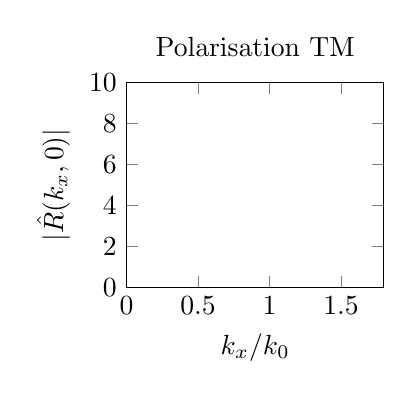
\begin{tikzpicture}[scale=1]
    \begin{axis}[
            title={Polarisation TM},
            ylabel={\(|\hat{R}(k_x,0)|\)},
            xlabel={\(k_x\slash k_0\)},
            width=0.4\textwidth,
            ymin=0,
            ymax=10,
            restrict y to domain=0:+4E+01,
            xmin=0,
            xmax=1.8,
            mark repeat=40,
            legend pos=outer north east
        ]
        % \addplot [color=black,mark=square*] table [col sep=comma, x={s1}, y={Abs(r_ex.tm)}] {csv/SOUDAIS/SOUDAIS.r_ex.MODE_2_TYPE_P.csv};
        % % \addlegendentry{Exact};

        % \addplot [color=blue,mark=x] table [col sep=comma, x={s1}, y={Abs(r_ibc0.tm)}] {csv/SOUDAIS/SOUDAIS.r_ibc.IBC_ibc0_SUC_F_MODE_2_TYPE_P.csv};
        % % \addlegendentry{CI0};

        % \addplot [color=red,mark=diamond*] table [col sep=comma, x={s1}, y={Abs(r_ibc3.tm)}] {csv/SOUDAIS/SOUDAIS.r_ibc.IBC_ibc3_SUC_F_MODE_2_TYPE_P.csv};
        % % \addlegendentry{CI3};
    \end{axis}
\end{tikzpicture}
\tikzsetnextfilename{R_SOUDAIS_plan_hoibc.TE}
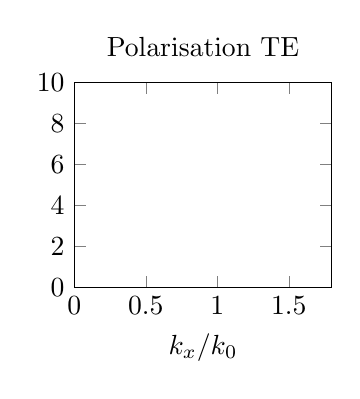
\begin{tikzpicture}[scale=1]
    \begin{axis}[
            title={Polarisation TE},
            ylabel={},
            xlabel={\(k_x\slash k_0\)},
            width=0.4\textwidth,
            xmin=0,
            xmax=1.8,
            ymin=0,
            ymax=10,
            mark repeat=40,
            legend pos=outer north east
        ]
        % \addplot [color=black,mark=square*] table [col sep=comma, x={s1}, y={Abs(r_ex.te)}] {csv/SOUDAIS/SOUDAIS.r_ex.MODE_2_TYPE_P.csv};
        % \addlegendentry{Exact};

        % \addplot [color=blue,mark=x] table [col sep=comma, x={s1}, y={Abs(r_ibc0.te)},color=] {csv/SOUDAIS/SOUDAIS.r_ibc.IBC_ibc0_SUC_F_MODE_2_TYPE_P.csv};
        % \addlegendentry{CI0};

        % \addplot [color=red,mark=diamond*] table [col sep=comma, x={s1}, y={Abs(r_ibc3.te)}] {csv/SOUDAIS/SOUDAIS.r_ibc.IBC_ibc3_SUC_F_MODE_2_TYPE_P.csv};
        % \addlegendentry{CI3};
    \end{axis}
\end{tikzpicture}
          \caption[CIOE sur empilement de P.~Soudais p.~11]{Module des coefficients diagonaux de \(\mR\) pour \(\eps = 4, \mu = 1, d=0.035\text{m}, f=12\text{GHz}\)}
          \label{fig:reflex_fourier:plan:soudais:hoibc}
      \end{figure}

      La figure \ref{fig:imp_fourier:plan:triple_asymptote:hoibc} montre la limite de la CI3 pour capturer 3 asymptotes. Pour cela, il faudrait utiliser une CI d'ordre au moins 6.

      L'expression de cette CIOE que l'on nomme \hyperlink{ci7}{CI7} est
      \begin{equation}
        \left(\oI + \sum_{i=1}^3 \left(d_{i} \left(\frac{\LD}{k_0^2}\right)^i + e_{i} \left(-\frac{\LR}{k_0^2}\right)^i \right)\right)\vE_t = \left(a_0 \oI + \sum_{i=1}^3 \left(b_{i} \left(\frac{\LD}{k_0^2}\right)^i + c_{i} \left(-\frac{\LR}{k_0^2}^i\right) \right)\right)\vJ
      \end{equation}

      \begin{figure}[!hbt]
          \centering
          \tikzsetnextfilename{Z_triple_asymptote_plan_hoibc_TM}
\begin{tikzpicture}[scale=1]
    \begin{axis}[
            title={Polarisation TM},
            ylabel={\(\Im(\hat{Z}(k_x,0)\)},
            xlabel={\(k_x\slash k_0\)},
            width=0.4\textwidth,
            xmin=0,
            xmax=1.999,
            ymin=-10,
            ymax=10,
            restrict y to domain=-300:300,
            mark repeat=200,
            legend pos=outer north east
        ]
        \addplot [color=black,mark=square*] table [col sep=comma, x={s1}, y={Im(z_ex.tm)}] {csv/triple_asymptote/triple_asymptote.z_ex.P.csv};
        % \addlegendentry{Exact};

        \addplot [color=blue,mark=x] table [col sep=comma, x={s1}, y={Im(z_ibc0.tm)}] {csv/triple_asymptote/triple_asymptote.z_ibc.IBC_ibc0_TYPE_P_SUC_F.csv};
        % \addlegendentry{CI0};

        \addplot [color=red,mark=diamond*] table [col sep=comma, x={s1}, y={Im(z_ibc3.tm)}] {csv/triple_asymptote/triple_asymptote.z_ibc.IBC_ibc3_TYPE_P_SUC_F.csv};
        % \addlegendentry{CI3};

        \addplot [color=cyan,mark=pentagon*] table [col sep=comma, x={s1}, y={Im(z_ibc7.tm)}] {csv/triple_asymptote/triple_asymptote.z_ibc.IBC_ibc7_TYPE_P_SUC_F.csv};
        % \addlegendentry{CI7};
    \end{axis}
\end{tikzpicture}
\tikzsetnextfilename{Z_triple_asymptote_plan_hoibc_TE}
\begin{tikzpicture}[scale=1]
    \begin{axis}[
            title={Polarisation TE},
            ylabel={},
            xlabel={\(k_x\slash k_0\)},
            width=0.4\textwidth,
            xmin=0,
            xmax=1.999,
            ymin=-10,
            ymax=10,
            restrict y to domain=-300:300,
            mark repeat=200,
            legend pos=outer north east
        ]
        \addplot [color=black,mark=square*] table [col sep=comma, x={s1}, y={Im(z_ex.te)}] {csv/triple_asymptote/triple_asymptote.z_ex.P.csv};
        \addlegendentry{Exact};

        \addplot [color=blue,mark=x] table [col sep=comma, x={s1}, y={Im(z_ibc0.te)}] {csv/triple_asymptote/triple_asymptote.z_ibc.IBC_ibc0_TYPE_P_SUC_F.csv};
        \addlegendentry{CI0};

        \addplot [color=red,mark=diamond*] table [col sep=comma, x={s1}, y={Im(z_ibc3.te)}] {csv/triple_asymptote/triple_asymptote.z_ibc.IBC_ibc3_TYPE_P_SUC_F.csv};
        \addlegendentry{CI3};

        \addplot [color=cyan,mark=pentagon*] table [col sep=comma, x={s1}, y={Im(z_ibc7.te)}] {csv/triple_asymptote/triple_asymptote.z_ibc.IBC_ibc7_TYPE_P_SUC_F.csv};
        \addlegendentry{CI7};                  
    \end{axis}
\end{tikzpicture}
          \caption[CIOE sur empilement avec triple asymptote]{Partie imaginaire des coefficients diagonaux de \(\mZ\) pour \(\eps = 4, \mu = 1, d=0.2\text{m}, f=1\text{GHz}\)}
          \label{fig:imp_fourier:plan:triple_asymptote:hoibc}
      \end{figure}
      \begin{table}[!hbt]
        \centering
        \begin{minipage}[t]{0.49\textwidth}
        \vspace{0pt}
        \centering
        \begin{coefftable}{\hyperlink{ci0}{CI0}}
          \input{csv/triple_asymptote/triple_asymptote.IBC_ibc0_SUC_F_MODE_2_TYPE_P.coeff.txt}
        \end{coefftable}

        \begin{coefftable}{\hyperlink{ci3}{CI3}}
          \input{csv/triple_asymptote/triple_asymptote.IBC_ibc3_SUC_F_MODE_2_TYPE_P.coeff.txt}
        \end{coefftable}
        \end{minipage}
        \tablecoeff[0.49]{\hyperlink{ci7}{CI7}}{csv/triple_asymptote/triple_asymptote.IBC_ibc7_SUC_F_MODE_2_TYPE_P.coeff.txt}
        \caption{Coefficients associés à la figure \ref{fig:imp_fourier:plan:triple_asymptote:hoibc}}
        \label{tab:imp_fourier:plan:triple_asymptote:hoibc}
      \end{table}
      Il faut donc une CIOE d'ordre 2 fois le nombre d'asymptote que l'on rencontre sur notre balayage.
\subsection{Problème de la singularité de l'impédance dans le cadre du plan infini pour une couche de matériau sans perte}

Dans la partie précédente nous avons introduit la fonctionnelle que l'on cherche à minimiser qui est \(F(X) = \left\lVert\tilde{\mH} X - b(\mZ_{ex})\right\rVert_{\RR^N}\).

On se place dans le cadre du plan infini de \cite{aubakirov_electromagnetic_2014}, où \(\eps=4,\mu=1,f=12\) Ghz, et \(d=3.5\) mm. %Ce cas non physique possède un onde guidée pour \((k_x,k_y) = (k_0s^\star,0.)\) où \(\mR(k_0s^\star,0.) = \infty\).

Il existe un \(s_z\) tel que \(\hat\mZ_{ex}(k_0s_z,0.) = \infty\). En effet, d'après la formule pour une couche de matériau \eqref{eq:imp_plan:symb_z:1c}, 

\begin{equation}
  \hat{\mZ}_{ex}(k_x,0.) = i\frac{\eta}{k\sqrt{k^2 - k_x^2}}\tan(\sqrt{k^2 - k_x^2}d)\left(k^2\mI - \hat{\mLR}\right)
\end{equation}
Donc il est facile de voir que l'on a une asymptote à cause de la tangente et donc pour cet empilement
\begin{equation}
  s_z = \sqrt{\eps \mu - \left(\frac{\pi/2}{k_0 d}\right)^2}
\end{equation}

Le problème est donc que si nous balayons en incidence et que l'on passe par ce point, alors la matrice \(\hat\mZ\) n'est pas défini en ce point. Or comme le gradient de la fonctionnelle est fonction de cette matrice, le gradient n'est pas défini pour tout \(X\). Si l'on utilise une méthode basée sur le gradient de type Newton, ce que nous avons fait, on comprend pourquoi la méthode numérique échoue à calculer des coefficients.

\subsubsection{Réduction du nombre de variables de la minimisation}

On décompose alors nos matrices et vecteurs en séparant les parties contentant cette asymptote.

On suppose donc qu'il existe \(\tilde{\mH}_\infty, \tilde{b}_\infty, X_\infty,\) tels que
\begin{align*}
  \tilde{\mH} &= \tilde{\mH}_\infty + \tilde{\mH}_r
  \\
  \tilde{b} &= \tilde{b}_\infty + \tilde{b}_r
  \\
  X &= X_\infty + X_r
\end{align*}

Ces matrices et vecteurs sont reliés par les relations
\begin{align}
  \tilde{\mH}_\infty X_\infty &= \tilde{b}_\infty
  \\
  \tilde{\mH}_\infty X_r &= 0
\end{align}

Il faut vraiment voir cette décomposition comme deux partie, où l'une est nulle quasiment partout sauf pour le \(s_z\) problématique et l'autre est définie normalement sauf aux termes correspondant au \(s_z\) où elle est nulle.

Schématiquement on définit \(i_z\) l'indice d'une ligne telle que \(\tilde{b}(\hat{\mZ})_{i_z} = \infty\)

\begin{equation*}
  \begin{matrix}
    \tilde{\mH} &=& \tilde{\mH}_\infty &+& \tilde{\mH}_r
    \\
    \begin{bmatrix}
      \tilde{\mH}_{1,1} & \cdots & \tilde{\mH}_{1,N_{CI}}
      \\
      \vdots & \ddots & \vdots
      \\
      \tilde{\mH}_{i_z-1,1} & \cdots & \tilde{\mH}_{i_z-1,N_{CI}}
      \\
      \tilde{\mH}_{i_z,1} & \cdots & \tilde{\mH}_{i_z,N_{CI}}
      \\
      \tilde{\mH}_{i_z+1,1} & \cdots & \tilde{\mH}_{i_z+1,N_{CI}}
      \\
      \vdots & \ddots & \vdots
      \\
      \tilde{\mH}_{4N_i,1} & \cdots & \tilde{\mH}_{4N_i,N_{CI}}
    \end{bmatrix}
    & = &
    \begin{bmatrix}
      0 & \cdots & 0
      \\
      \vdots & \ddots & \vdots
      \\
      0 & \cdots & 0
      \\
      \tilde{\mH}_{i_z,1} & \cdots & \tilde{\mH}_{i_z,N_{CI}}
      \\
      0 & \cdots & 0
      \\
      \vdots & \ddots & \vdots
      \\
      0 & \cdots & 0
    \end{bmatrix}
    & + & 
    \begin{bmatrix}
      \tilde{\mH}_{1,1} & \cdots & \tilde{\mH}_{1,N_{CI}}
      \\
      \vdots & \ddots & \vdots
      \\
      \tilde{\mH}_{i_z-1,1} & \cdots & \tilde{\mH}_{i_z-1,N_{CI}}
      \\
      0 & \cdots & 0
      \\
      \tilde{\mH}_{i_z+1,1} & \cdots & \tilde{\mH}_{i_z+1,N_{CI}}
      \\
      \vdots & \ddots & \vdots
      \\
      \tilde{\mH}_{4N_i,1} & \cdots & \tilde{\mH}_{4N_i,N_{CI}}
    \end{bmatrix}
  \end{matrix}
\end{equation*}
Dans les fait, \(\tilde{\mH}_\infty\) à \(4\) lignes non-nulles et \(\tilde{\mH}_r\) en a autant de nulles au même endroits.


On développe donc la fonctionnelle suivant cette décomposition.
\begin{align*}
\argmin{X}\left\rVert \tilde{\mH} X - \tilde{b} \right \rVert &= \argmin{X_r}\left\rVert \left(\tilde{\mH}_\infty + \tilde{\mH}_r\right)\left( X_\infty + X_r \right) - \tilde{b}_\infty - \tilde{b}_r \right \rVert
\\
\intertext{On utilise la relation entre \(\tilde{\mH}_\infty X_\infty\) et \(\tilde{b}_\infty\)}
&=  \argmin {X_r}\left\rVert \tilde{\mH}_\infty X_r + \tilde{\mH}_r X_\infty + \tilde{\mH}_r X_r - \tilde{b}_r \right \rVert
\\
\intertext{Enfin par définition de \(\tilde{\mH}_\infty\) et \(X_r\), leur produit est nul}
&= \argmin{X_r} \left\rVert \tilde{\mH}_r ( X_r + X_\infty)- \tilde{b}_r \right \rVert
\end{align*}

On voit alors que l'on peut résoudre le problème si l'on minimise uniquement sur les \(X_r\), les autres étant fixés et que l'on enlève du système les lignes où l'impédance n'est pas définie.

\subsubsection{Application de la réduction à la CI3}

On rappelle l'expression de la CI3
\begin{equation}
  \hat{\mZ}_{ap}(k_x,0.) = \left(\mI + b_1 \hat{\mLD} - b_2 \hat{\mLR} \right)^{-1}\left(a_0\mI + a_1 \hat{\mLD} - a_2 \hat{\mLR} \right)
\end{equation}

On voit donc que pour faire apparaître une asymptote, il faut que la matrice de gauche ne soit pas inversible en \(s_z\).

La matrice \(\tilde{\mH}_\infty\) est donc nulle partout sauf en 8 termes, placés sur les deux dernières colonnes et les 4 lignes correspondantes à \((k_x,k_y)=(k_0 s_z,0)\).

Connaissant les expressions des matrices \(\hat\mLD,\hat\mLR\) introduites dans la partie précédente alors on déduit que
\begin{align}
  X_\infty = \begin{bmatrix}
    0\\
    0\\
    0\\
    (k_0 s_z)^{-2}\\
    (k_0 s_z)^{-2}\\
  \end{bmatrix}
  & &
  X_r = \begin{bmatrix}
  a_0\\
  a_1\\
  a_2\\
  0\\
  0\\
  \end{bmatrix}
\end{align}

\subsection{Choix de la méthode numérique pour résoudre la minimisation sous contraintes}

  Des méthodes basées sur le gradient sont adaptées car la fonctionnelle est dérivable pour tout \(X\) et les contraintes se comportent comme des polynômes dépendant uniquement des composantes de \(X\). Nous avons donc fait le choix de la méthode \gls{acr-sqp} pour les raisons suivantes:
 
  \begin{itemize}
    \item Elle est éprouvée depuis \cite{kraft_software_1988} et des sources Fortran à jour sont disponibles à \url{https://github.com/jacobwilliams/slsqp}, ce qui est capital pour l'intégrer dans un code industriel.
    \item Elle est rapide, nous avons observés que cette méthode convergeait en quelques dizaines d'itérations au pire.
    \item Elle accepte des contraintes non-linaire donc elle est adaptée à nos CSU.
  \end{itemize}

\subsection{Résultats numérique avec contraintes}

  \begin{TODO}
    Quelques résultats avec contraintes
  \end{TODO}
\section{Calcul des coefficients de la CI3 par moindres carrés sur les coefficients de la série de Fourier}

  On peut aussi calculer les coefficients en minimisant l'erreur entre les coefficients de Fourier.

  Soit \(\mM_A\) et \(\mM_B\) les fonctions introduites à la définition \ref{def:plan:matrices_MA-MB} et \(\hat\mR\) la fonction définie en \ref{def:plan:reflexion:impedance}.

  \begin{defn}%[]
    \label{def:plan:minimisation:matrices_MR}
    On définit les fonctions \(\hat\mR_{ex}, \hat\mR_{CI3}\) de \(\RR\times\RR\times \rightarrow \mathcal{M}_2(\CC)\) telles que
    \begin{align*}
      \hat\mR_{ex}(k_x,k_y) &= \hat\mR(k_x,k_y, \hat\mZ_{ex}(k_x,k_y)),
      \\
      \hat\mR_{CI3}(k_x,k_y) &= \hat\mR(k_x,k_y, \hat\mZ_{CI3}(k_x,k_y)).
    \end{align*}
    où \(\hat\mZ_{ex},\hat\mZ_{CI3}\) sont des fonctions définies à la proposition \ref{prop:plan:synthese:impedance} et à l'équation \eqref{eq:plan:hoibc:ci3}.
  \end{defn}

  \subsection[Expression de la fonction JR]{Expression de la fonction \(J_R\)}

    On utilise les fonctions \(\mN_E, \mN_H\) introduites à la définition \ref{def:plan:matrices_NE-NH} et \(\hat\mLD,\hat\mLR\) définies aux définitions \ref{eq:plan:fourier:LD}-\ref{eq:plan:fourier:LR}.

    \begin{defn}
      On définit \(\mA_0,\mA_1,\mA_2,\mA_2,\mB_1,\mB_2\) les fonctions de \(\RR \times \RR \times \mathcal{M}_2(\CC) \rightarrow \ \mathcal{M}_2(\CC)\) telles que        
      \begin{align*}
        \mA_0(k_x,k_y,\mR) &= \mN_E(k_x,k_y,0^+,\mR),
        \\
        \mA_1(k_x,k_y,\mR) &= \hat{\mLD}(k_x,k_y)\mN_E(k_x,k_y,0^+,\mR),
        \\
        \mA_2(k_x,k_y,\mR) &= -\hat{\mLR}(k_x,k_y)\mN_E(k_x,k_y,0^+,\mR),
        \\
        \mB_1(k_x,k_y,\mR) &= \hat{\mLD}(k_x,k_y)\mN_H(k_x,k_y,0^+,\mR),
        \\
        \mB_2(k_x,k_y,\mR) &= -\hat{\mLR}(k_x,k_y)\mN_H(k_x,k_y,0^+,\mR).            
      \end{align*}

      On définit \(\tilde{\mH}_{CI3}\) la fonction de \(\RR \times \RR \times \mathcal{M}_2(\CC) \rightarrow \mathcal{M}_{4\times5}(\CC)\) telle que
      \begin{align*}
        & \tilde\mH_{CI3}(k_x,k_y,\mR) =  \\ &
        \begin{bmatrix}
          \mA_0(k_x,k_y,\mR)_{11} & \mA_1(k_x,k_y,\mR)_{11} & \mA_2(k_x,k_y,\mR)_{11} & \mB_1(k_x,k_y,\mR)_{11} & \mB_2(k_x,k_y,\mR)_{11}
          \\
          \mA_0(k_x,k_y,\mR)_{12} & \mA_1(k_x,k_y,\mR)_{12} & \mA_2(k_x,k_y,\mR)_{12} & \mB_1(k_x,k_y,\mR)_{12} & \mB_2(k_x,k_y,\mR)_{12}
          \\
          \mA_0(k_x,k_y,\mR)_{21} & \mA_1(k_x,k_y,\mR)_{21} & \mA_2(k_x,k_y,\mR)_{21} & \mB_1(k_x,k_y,\mR)_{21} & \mB_2(k_x,k_y,\mR)_{21}
          \\
          \mA_0(k_x,k_y,\mR)_{22} & \mA_1(k_x,k_y,\mR)_{22} & \mA_2(k_x,k_y,\mR)_{22} & \mB_1(k_x,k_y,\mR)_{22} & \mB_2(k_x,k_y,\mR)_{22}
        \end{bmatrix}.
      \end{align*}

      On définit \(\tilde{b}\) la fonction de \(\RR \times \RR \times \mathcal{M}_2(\CC) \rightarrow \CC^4\) telle que
      \begin{equation*}
        \tilde{b}(k_x,k_y,\mR) = -
        \begin{bmatrix}
          \mN_H(k_x,k_y,0^+,\mR)_{11}
          \\
          \mN_H(k_x,k_y,0^+,\mR)_{12}
          \\
          \mN_H(k_x,k_y,0^+,\mR)_{21}
          \\
          \mN_H(k_x,k_y,0^+,\mR)_{22}
        \end{bmatrix}.
      \end{equation*}
    \end{defn}

    \begin{prop}
      Soit \(X = (a_0,a_1,a_2,b_1,b_2)\), \((k_x,k_y)\) fixé et \(\hat\mR_{ex}\) la matrice définie en \ref{def:plan:minimisation:matrices_MR}, alors
      \begin{multline*}
        \argmin{X\in\CC^5} \norm{\hat\mR_{CI3}(k_x,k_y,X) - \hat\mR_{ex}(k_x,k_y)} =
        \\
        \argmin{X\in\CC^5} \norm{\tilde{\mH}_{CI3}(k_x,k_y,\hat\mR_{ex}(k_x,k_y))X - \tilde{b}(k_x,k_y,\hat\mR_{ex}(k_x,k_y))}.
      \end{multline*}
    \end{prop}

    \begin{proof}
      C'est la même méthodologie que pour l'impédance.
      On rappelle de la section précédente
      \begin{multline*}
        \hat{\mZ}_{CI3}(k_x,k_y) = \left(\mI + b_1 \hat{\mLD}(k_x,k_y) - b_2 \hat{\mLR}(k_x,k_y) \right)^{-1}
        \\
        \left(a_0 \mI + a_1 {\hat{\mLD}(k_x,k_y)} - a_2 {\hat{\mLR}(k_x,k_y)}\right).
      \end{multline*}
      On pose \(\hat\mZ_D(k_x,k_y) = \mI + b_1 \hat{\mLD}(k_x,k_y) - b_2 \hat{\mLR}(k_x,k_y)\) et \(\hat\mZ_N(k_x,k_y) = a_0 \mI + a_1 {\hat{\mLD}(k_x,k_y)} - a_2 {\hat{\mLR}(k_x,k_y)}\) donc

      \begin{align*}
        &{\hspace{1em}}~ \argmin{X\in\CC^5} \norm{\hat\mR_{CI3}(k_x,k_y,X) - \hat\mR_{ex}(k_x,k_y)}
        \\
        & = \argmin{X\in\CC^5} \norm{ - \mM_B(k_x,k_y,0^+,\hat\mZ_{CI3})^{-1}\mM_A(k_x,k_y,0^+,\hat\mZ_{CI3})- \hat\mR_{ex}(k_x,k_y) },
        \\
        & = \argmin{X\in\CC^5} \norm{ - \mM_B(k_x,k_y,0^+,\hat\mZ_{CI3})^{-1}\left(\mM_A(k_x,k_y,0^+,\hat\mZ_{CI3}) +  \mM_B(k_x,k_y,0^+,\hat\mZ_{CI3})\hat\mR_{ex}(k_x,k_y)\right) },    
        \\ 
        & = \argmin{X\in\CC^5} \norm{\mM_A(k_x,k_y,0^+,\hat\mZ_{CI3}) +\mM_B(k_x,k_y,0^+,\hat\mZ_{CI3})\hat\mR_{ex}(k_x,k_y)}.
        \intertext{D'après la définition \ref{def:plan:matrices_MA-MB} des fonctions \(\mM_A, \mM_B\),}
        & = \argmin{X\in\CC^5} \left\lVert \left(\mJ_E(k_x,k_y,0^+)-\hat\mZ_{CI3}(k_x,k_y)\mJ_H(k_x,k_y,0^+)\right) \right.
        \\
        & \qquad \qquad \quad + \left.\left(\mH_E(k_x,k_y,0^+)-\hat\mZ_{CI3}(k_x,k_y)\mH_H(k_x,k_y,0^+)\right)\hat\mR_{ex}(k_x,k_y) \right\lVert.
        \intertext{D'après la définition de \(\hat\mZ_{CI3}\),}        
        & = \argmin{X\in\CC^5} \left\lVert \hat\mZ_D(k_x,k_y)^{-1}\left(\hat\mZ_D(k_x,k_y)\mJ_E(k_x,k_y,0^+)-\hat\mZ_N(k_x,k_y)\mJ_H(k_x,k_y,0^+)\right) \right.
        \\
        & \qquad \qquad \quad + \left.\hat\mZ_D(k_x,k_y)^{-1}\left(\hat\mZ_D(k_x,k_y)\mH_E(k_x,k_y,0^+)-\hat\mZ_N(k_x,k_y)\mH_H(k_x,k_y,0^+)\right)\hat\mR_{ex}(k_x,k_y) \right\lVert,
        \\
        & = \argmin{X\in\CC^5} \left\lVert \left(\hat\mZ_D(k_x,k_y)\mJ_E(k_x,k_y,0^+)-\hat\mZ_N(k_x,k_y)\mJ_H(k_x,k_y,0^+)\right) \right.
        \\
        & \qquad \qquad \quad + \left.\left(\hat\mZ_D(k_x,k_y)\mH_E(k_x,k_y,0^+)-\hat\mZ_N(k_x,k_y)\mH_H(k_x,k_y,0^+)\right)\hat\mR_{ex}(k_x,k_y) \right\lVert.
        \intertext{D'après la définition \ref{def:plan:matrices_NE-NH} des fonctions \(\mN_E, \mN_H\),}        
        & = \argmin{X\in\CC^5} \norm{\hat\mZ_N(k_x,k_y)\mN_E(k_x,k_y,0^+,\hat\mR_{ex}(k_x,k_y)) + \hat\mZ_D(k_x,k_y)\mN_H(k_x,k_y,0^+,\hat\mR_{ex}(k_x,k_y))}.
      \end{align*}
      et l’on conclut d'après la définition des fonctions \(\hat\mZ_D, \hat\mZ_N\).
    \end{proof}

    \begin{defn}
      On définit \(\tilde{\mA}_{CI3}\) la matrice de \(\mathcal{M}_{4N_{n}N_{k_z}\times5}(\CC)\) telle que
      \begin{equation*}
        \tilde{\mA}_{CI3} = 
        \begin{bmatrix}
          \tilde\mH_{CI3}(n_1,k_{z1},\hat\mR_{ex}(n_1,k_{z1}))
          \\
          \vdots
          \\
          \tilde\mH_{CI3}(n_i,k_{zj},\hat\mR_{ex}(n_i,k_{zj}))
          \\
          \vdots
          \\
          \tilde\mH_{CI3}(n_{N_n},k_{zN_{k_z}},\hat\mR_{ex}(n_{N_n},k_{zN_{k_z}}))
        \end{bmatrix}.
      \end{equation*}
      On définit \(\tilde{g}\) le vecteur colonne \(\CC^{4N_{n}N_{k_z}}\) telle que
      \begin{equation*}
        \tilde{g} = 
        \begin{bmatrix}
          \tilde{b}(n_1,k_{z1},\hat\mR_{ex}(n_1,k_{z1}))
          \\
          \vdots
          \\
          \tilde{b}(n_i,k_{zj},\hat\mR_{ex}(n_i,k_{zj}))
          \\
          \vdots
          \\
          \tilde{b}(n_{N_n},k_{zN_{k_z}},\hat\mR_{ex}(n_{N_n},k_{zN_{k_z}}))
        \end{bmatrix}.
      \end{equation*}
    \end{defn}

    On peut alors calculer les coefficients de la CI3

    \begin{defn}
      On définit la fonction \(J_R\)
      \begin{equation*}
        J_R(X) = \norm{\tilde{\mA}_{CI3}X - \tilde{g}}.
      \end{equation*}
    \end{defn}
    \begin{REM}
      Je mettrai on introduit, et pas une définition
    \end{REM}
    \begin{REP}
      Ok, mais je peux qu'on puisse bien la voir, pour ne pas confondre avec JZ
    \end{REP}
    \begin{thm}[Minimisation sans contraintes pour la CI3]

      Les coefficients de la CIOE sont solutions du problème

      Trouver \(X^* \in \CC^5\) tel que
      \begin{equation*}
        X^* = \argmin{X\in \CC^5} J_R(X).
      \end{equation*}
    \end{thm}

    \begin{prop}
      Si \(\conj{\tilde{\mA}_{CI3}^t}\tilde{\mA}_{CI3}\) est inversible, alors
      \begin{equation*}
        X^* = (\conj{\tilde{\mA}_{CI3}^t}\tilde{\mA}_{CI3})^{-1}\conj{\tilde{\mA}_{CI3}^t}\tilde{g}.
      \end{equation*}
    \end{prop}
    \begin{proof}
      Même méthode que pour la proposition \ref{prop:plan:minimisation:minimum_sans_contraintes} sur l'impédance.
    \end{proof}

    Nous n'avons pas réussi à démontrer que cette matrice était définie pour tout empilement et toute incidence, pas même pour des CIOE plus simples.

    \begin{thm}[Minimisation avec contraintes pour la CI3]

      Soit \(\CSU[3]{CI3}\) le sous-espace de \(\CC^5\) issu de la définition \ref{def:csu:ci3-3}, alors les coefficients de la CIOE respectant les CSU sont solutions du problème

      Trouver \(X^* \in \CC^5\) tel que
      \begin{equation*}
        X^* = \argmin{X\in \CSU[3]{CI3}} J_R(X).
      \end{equation*}
    \end{thm}

    


\sectionstar{Conclusion}
Nous avons montré comment calculer les coefficients dans le cas d'un objet plan infini en minimisant au sens des moindres carrés la différence entre les matrices d'impédance exactes et approchées et  nous pouvons aussi minimiser l'erreur entre les matrices de réflexion, mais cela n'apporte rien.

Pour cela, nous avons réalisé une analyse spectrale des équations de Maxwell et montré que la condition d'impédance s'exprime comme un multiplicateur de Fourier matriciel, tout comme la matrice de réflexion. Grâce à cette analyse spectrale, nous avons aussi exprimé les CIOE comme des multiplicateurs de Fourier matriciels dont on a déduit la matrice de réflexion associée. Nous avons alors exprimé le problème de minimisation sous contraintes et montré que celui-ci a besoin d'être réduit dans le cas d'une couche de matériau sans pertes.

Nous avons montré sur cette géométrie que la CIOE choisie, la \hyperlink{ci3}{CI3}, était largement plus précise que les précédentes \hyperlink{ci01}{CI01} et \hyperlink{ci1}{CI1}. Ce gain en précision est tel que l'on peut introduire des contraintes lors du calcul et avoir une solution finale convenable, relativement à l'opérateur exact.

Dans la partie équation intégrale, nous verrons que cette approximation locale de la géométrie est souvent suffisante.
